\documentclass[11pt]{article}

% --- Packages ---
\usepackage[margin=1in]{geometry}
\usepackage{graphicx}
\usepackage{booktabs}
\usepackage{amsmath,amssymb}
\usepackage{natbib}
\usepackage{hyperref}
\usepackage{xcolor}
\usepackage{multirow}
\usepackage{caption}
\usepackage{subcaption}
\usepackage{enumitem}
\usepackage{microtype}

% --- Metadata ---
\title{Semantic Drift in the Qwen3.5 Model Family:\\
Scaling, Quantization, Temperature, and Prompt Engineering}

\author{
  James H.\ Smith \\
  Joshua.AI LLC \\
  \texttt{jim@joshua8.ai}
}

\date{March 2026}

\begin{document}
\maketitle

% =============================================================================
% ABSTRACT
% =============================================================================
\begin{abstract}
We extend the semantic drift framework of \citet{smith2026semantic} to the
Qwen3.5 model family, conducting a controlled within-family analysis across
18 GGUF models (0.8B--122B parameters, 7 sizes and 18 size/quant
combinations), an AWQ and a GPTQ-Int4 variant of the 35B MoE served via
vLLM, an NVFP4 variant served via sglang, a 9B AWQ variant, and an
out-of-family Nemotron-3-Nano-30B NVFP4 control.
Across 1{,}969 completed 30-iteration chains comprising 59{,}070 LLM
inferences, we investigate four research questions:
\textbf{RQ1}~how drift varies with model size and quantization,
\textbf{RQ2}~whether GGUF, AWQ, NVFP4, and GPTQ-Int4 quantization produce
different drift dynamics for the same 35B MoE architecture,
\textbf{RQ3}~how sampling temperature interacts with model size, and
\textbf{RQ4}~whether system prompt effects generalize across model sizes
and quantization formats.
Key findings include:
(1)~a stability threshold at approximately 4B parameters, below which drift
becomes unpredictable;
(2)~quantization effects that are non-monotonic and size-dependent---BF16
does not always outperform Q4\_K\_M;
(3)~clear differences between 4-bit quantization \emph{methods} for the same
35B MoE architecture, although the per-method confidence intervals overlap
at $n\leq5$ chains per cell;
(4)~inverted temperature sensitivity in smaller models.
A cross-generation comparison with Qwen3 at matched parameter counts is
also reported, with the caveat that the Qwen3 arm comes from single
unreplicated pilot runs.
\end{abstract}

% =============================================================================
% 1. INTRODUCTION
% =============================================================================
\section{Introduction}
\label{sec:intro}

In \citet{smith2026semantic} (hereafter ``Paper~1''), we established a
telephone-game framework for measuring semantic drift in iterated LLM
paraphrase chains. That study examined 17 diverse models, KV cache precision
effects, system prompts, and temperature, finding a stable four-tier model
hierarchy, non-monotonic infrastructure effects, and a complexity threshold
for prompt engineering.

Paper~1 compared models \emph{across} families---Qwen3, Gemma3, Llama~3.1,
Devstral, GLM, and others---making it difficult to disentangle model-family
effects from size and quantization effects. The present study addresses this
limitation by conducting a controlled \emph{within-family} analysis of the
Qwen3.5 model family, holding architecture constant while varying size
(0.8B--122B), quantization (BF16, Q8\_0, Q4\_K\_M), serving backend
(Ollama GGUF vs.\ vLLM AWQ), temperature, and system prompts.

Our contributions are:
\begin{enumerate}[leftmargin=*]
  \item A systematic scaling analysis across 7 Qwen3.5 model sizes at 3
        quantization levels, revealing a stability threshold and non-monotonic
        quantization effects (Section~\ref{sec:rq1}).
  \item A controlled four-way comparison of GGUF, AWQ, NVFP4, and GPTQ-Int4
        quantization for the same 35B MoE architecture
        (Section~\ref{sec:rq2}).
  \item A temperature ablation across 5 model sizes showing inverted
        sensitivity in small models (Section~\ref{sec:rq3}).
  \item A system prompt ablation across six Qwen3.5 configurations and one
        out-of-family control, testing whether Paper~1's prompt engineering
        findings generalize within a single model family
        (Section~\ref{sec:rq4}).
  \item A cross-generation comparison between Qwen3 and Qwen3.5 at matched
        parameter counts (Section~\ref{sec:crossgen}).
\end{enumerate}

% =============================================================================
% 2. RELATED WORK
% =============================================================================
\section{Related Work}
\label{sec:related}

We refer readers to Paper~1 \citep{smith2026semantic} for a comprehensive
review of semantic drift, cultural attractors \citep{perez2025cultural,
brinkmann2023machine}, iterative generation distortion
\citep{mohamed2025broken}, agent drift \citep{rath2026agent}, attractor
cycles \citep{wang2025attractor, chytas2025concept}, and quantization
effects \citep{han2026quantization, hooper2024kvquant, liu2024kivi}.

The present study extends this literature by providing the first
controlled within-family scaling analysis of semantic drift. While Paper~1
demonstrated that model choice dominates infrastructure and prompt
engineering, it left open whether this hierarchy holds when architecture is
controlled. The Qwen3.5 family is well-suited for this analysis: it spans
two orders of magnitude in parameter count (0.8B--122B), includes both
dense and mixture-of-experts architectures, and is available in multiple
quantization formats across serving backends.

% =============================================================================
% 3. METHODOLOGY
% =============================================================================
\section{Methodology}
\label{sec:method}

\subsection{Experimental Framework}

We reuse the telephone-game framework from Paper~1: a single text is
paraphrased 30 times in sequence by the same model (``paraphrase'' prompt
style), with cosine similarity to the original measured at each iteration
using Qwen3-Embedding-0.6B. All experiments use 5 random seeds
$\{42, 137, 256, 512, 1024\}$ unless otherwise noted. Temperature is 0.7
by default.

\subsection{Prompts}

We use the same two prompts as Paper~1:
\begin{itemize}[leftmargin=*]
  \item \textbf{Spaghetti} (3 steps): ``Step~1: Boil water. Step~2: Add
        pasta for 8 minutes. Step~3: Drain and serve with sauce.''
  \item \textbf{Lasagna} (21 steps): A detailed homemade beef lasagna
        recipe with ingredients, measurements, and layering instructions
        (see Appendix~\ref{app:prompts}).
\end{itemize}

\subsection{Model Inventory}

Table~\ref{tab:models} summarizes the 22 Qwen3.5 model configurations
tested, together with one out-of-family control model.

\begin{table}[h]
\centering
\caption{Model inventory. GGUF models were served with Ollama; the AWQ and
  GPTQ-Int4 variants with vLLM; the NVFP4 variants with sglang. The
  Nemotron-3-Nano-30B row is an out-of-family control, included to test
  whether the RQ4 prompt rankings are specific to the Qwen3.5 family.
  See Appendix~\ref{app:compute} for hardware and software versions.}
\label{tab:models}
\small
\begin{tabular}{llll}
\toprule
Size & Architecture & Quantizations & Backend \\
\midrule
0.8B & Dense & Q8\_0, BF16 & Ollama \\
2B & Dense & Q4\_K\_M, Q8\_0, BF16 & Ollama \\
4B & Dense & Q4\_K\_M, Q8\_0, BF16 & Ollama \\
9B & Dense & Q4\_K\_M, Q8\_0, BF16 & Ollama \\
27B & Dense & Q4\_K\_M, Q8\_0, BF16 & Ollama \\
35B & MoE (A3B) & Q4\_K\_M, Q8\_0, BF16 & Ollama \\
35B & MoE (A3B) & AWQ 4-bit & vLLM \\
35B & MoE (A3B) & NVFP4 4-bit & sglang \\
35B & MoE (A3B) & GPTQ-Int4 & vLLM \\
9B & Dense & AWQ 4-bit & vLLM \\
122B & MoE & Q4\_K\_M & Ollama \\
\midrule
\multicolumn{4}{l}{\emph{Out-of-family control}} \\
30B & MoE (A3B) & NVFP4 4-bit & sglang \\
\bottomrule
\end{tabular}
\end{table}

\subsection{Experiments}

\begin{enumerate}[leftmargin=*]
  \item \textbf{Exp~1: Size $\times$ Quantization} (18 models $\times$ 2
        recipes $\times$ 5 seeds = 180 conditions).
  \item \textbf{Exp~2: Temperature ablation} (4 Ollama models $\times$ 2
        recipes $\times$ 5 temperatures $\times$ seeds = 168 conditions).
  \item \textbf{Exp~3: vLLM AWQ (35B MoE)} --- (a)~baseline drift
        (10 conditions), (b)~temperature ablation (42 conditions),
        (c)~system prompt ablation (200 conditions).
  \item \textbf{Exp~3d: sglang NVFP4 (35B MoE)} --- drift baseline
        (10 conditions), temperature ablation (42 conditions) and system
        prompt ablation (200 conditions).
  \item \textbf{Exp~3e: vLLM GPTQ-Int4 (35B MoE)} --- drift baseline
        (10 conditions), temperature ablation (42 conditions) and system
        prompt ablation (200 conditions).
  \item \textbf{Exp~3f: vLLM AWQ (9B dense)} --- drift baseline
        (10 conditions), temperature ablation (42 conditions) and system
        prompt ablation (200 conditions).
  \item \textbf{Exp~3g: sglang NVFP4 (Nemotron-3-Nano-30B, control)} ---
        drift baseline (10 conditions), temperature ablation
        (42 conditions) and system prompt ablation (200 conditions).
  \item \textbf{Exp~4: System prompt ablation} (2 Ollama models $\times$ 2
        recipes $\times$ 20 prompts $\times$ 5 seeds = 400 conditions).
\end{enumerate}

Counting only chains that completed all 30 iterations, the study comprises
1{,}969 conditions and $1{,}969 \times 30 = 59{,}070$ LLM inferences.

\paragraph{Data completeness.}
Of the 2{,}007 chains launched, 1{,}969 (98.1\%) ran to iteration~30 and are
the only chains used in any statistic reported here; partial chains are
neither padded nor silently averaged in, and every table reports the actual
$n$ behind each cell. The shortfalls are:
\begin{itemize}[leftmargin=*]
  \item \textbf{Exp~1}: 179/180. The condition
        \texttt{qwen3.5:35b-q4\_K\_M\_s256} (spaghetti) was never recorded,
        so the 35B MoE Q4\_K\_M spaghetti row rests on $n=4$.
  \item \textbf{Exp~3b} (AWQ temperature): 37/42, and \textbf{Exp~3c}
        (AWQ system prompts): 194/200. Eleven conditions were destroyed by a
        failed recovery run that replaced the original chains with
        zero-iteration error records. The AWQ endpoint was subsequently
        retired and these conditions could not be regenerated.
  \item \textbf{Exp~4}: 378/400. Nineteen of the 22 incomplete chains are
        27B lasagna conditions for prompts 15--20, lost when the Ollama
        serving host was decommissioned during a recovery run; the affected
        prompt cells therefore carry $n$ between 0 and 4, and one cell
        (27B lasagna, ``Balanced Clarity'') has no completed chain at all
        and is reported as absent rather than estimated. The remaining
        three are 9B lasagna chains that stopped at 15--23 iterations.
  \item \textbf{Exp~2 (Nemotron)}: 40/42; and one system-prompt chain each
        for NVFP4, GPTQ-Int4 and 9B~AWQ stopped between iterations 27
        and 29.
\end{itemize}

\subsection{Statistical Methods}

Following Paper~1, we report bootstrap 95\% confidence intervals
($B = 10{,}000$), Kruskal--Wallis $H$ with Dunn's post-hoc test
(Bonferroni-corrected) for tier comparisons, Wilcoxon signed-rank tests
for paired comparisons, Spearman rank correlations with bootstrap CIs for
cross-model prompt rankings, and Cohen's $d$ for effect sizes.

% =============================================================================
% 4. RESULTS
% =============================================================================
\section{Results}
\label{sec:results}

\subsection{RQ1: Size and Quantization}
\label{sec:rq1}

Figure~\ref{fig:lines} shows drift trajectories for all 18 Ollama models
on the spaghetti recipe. Table~\ref{tab:size_quant} provides
summary statistics.

\begin{figure}[t]
\centering
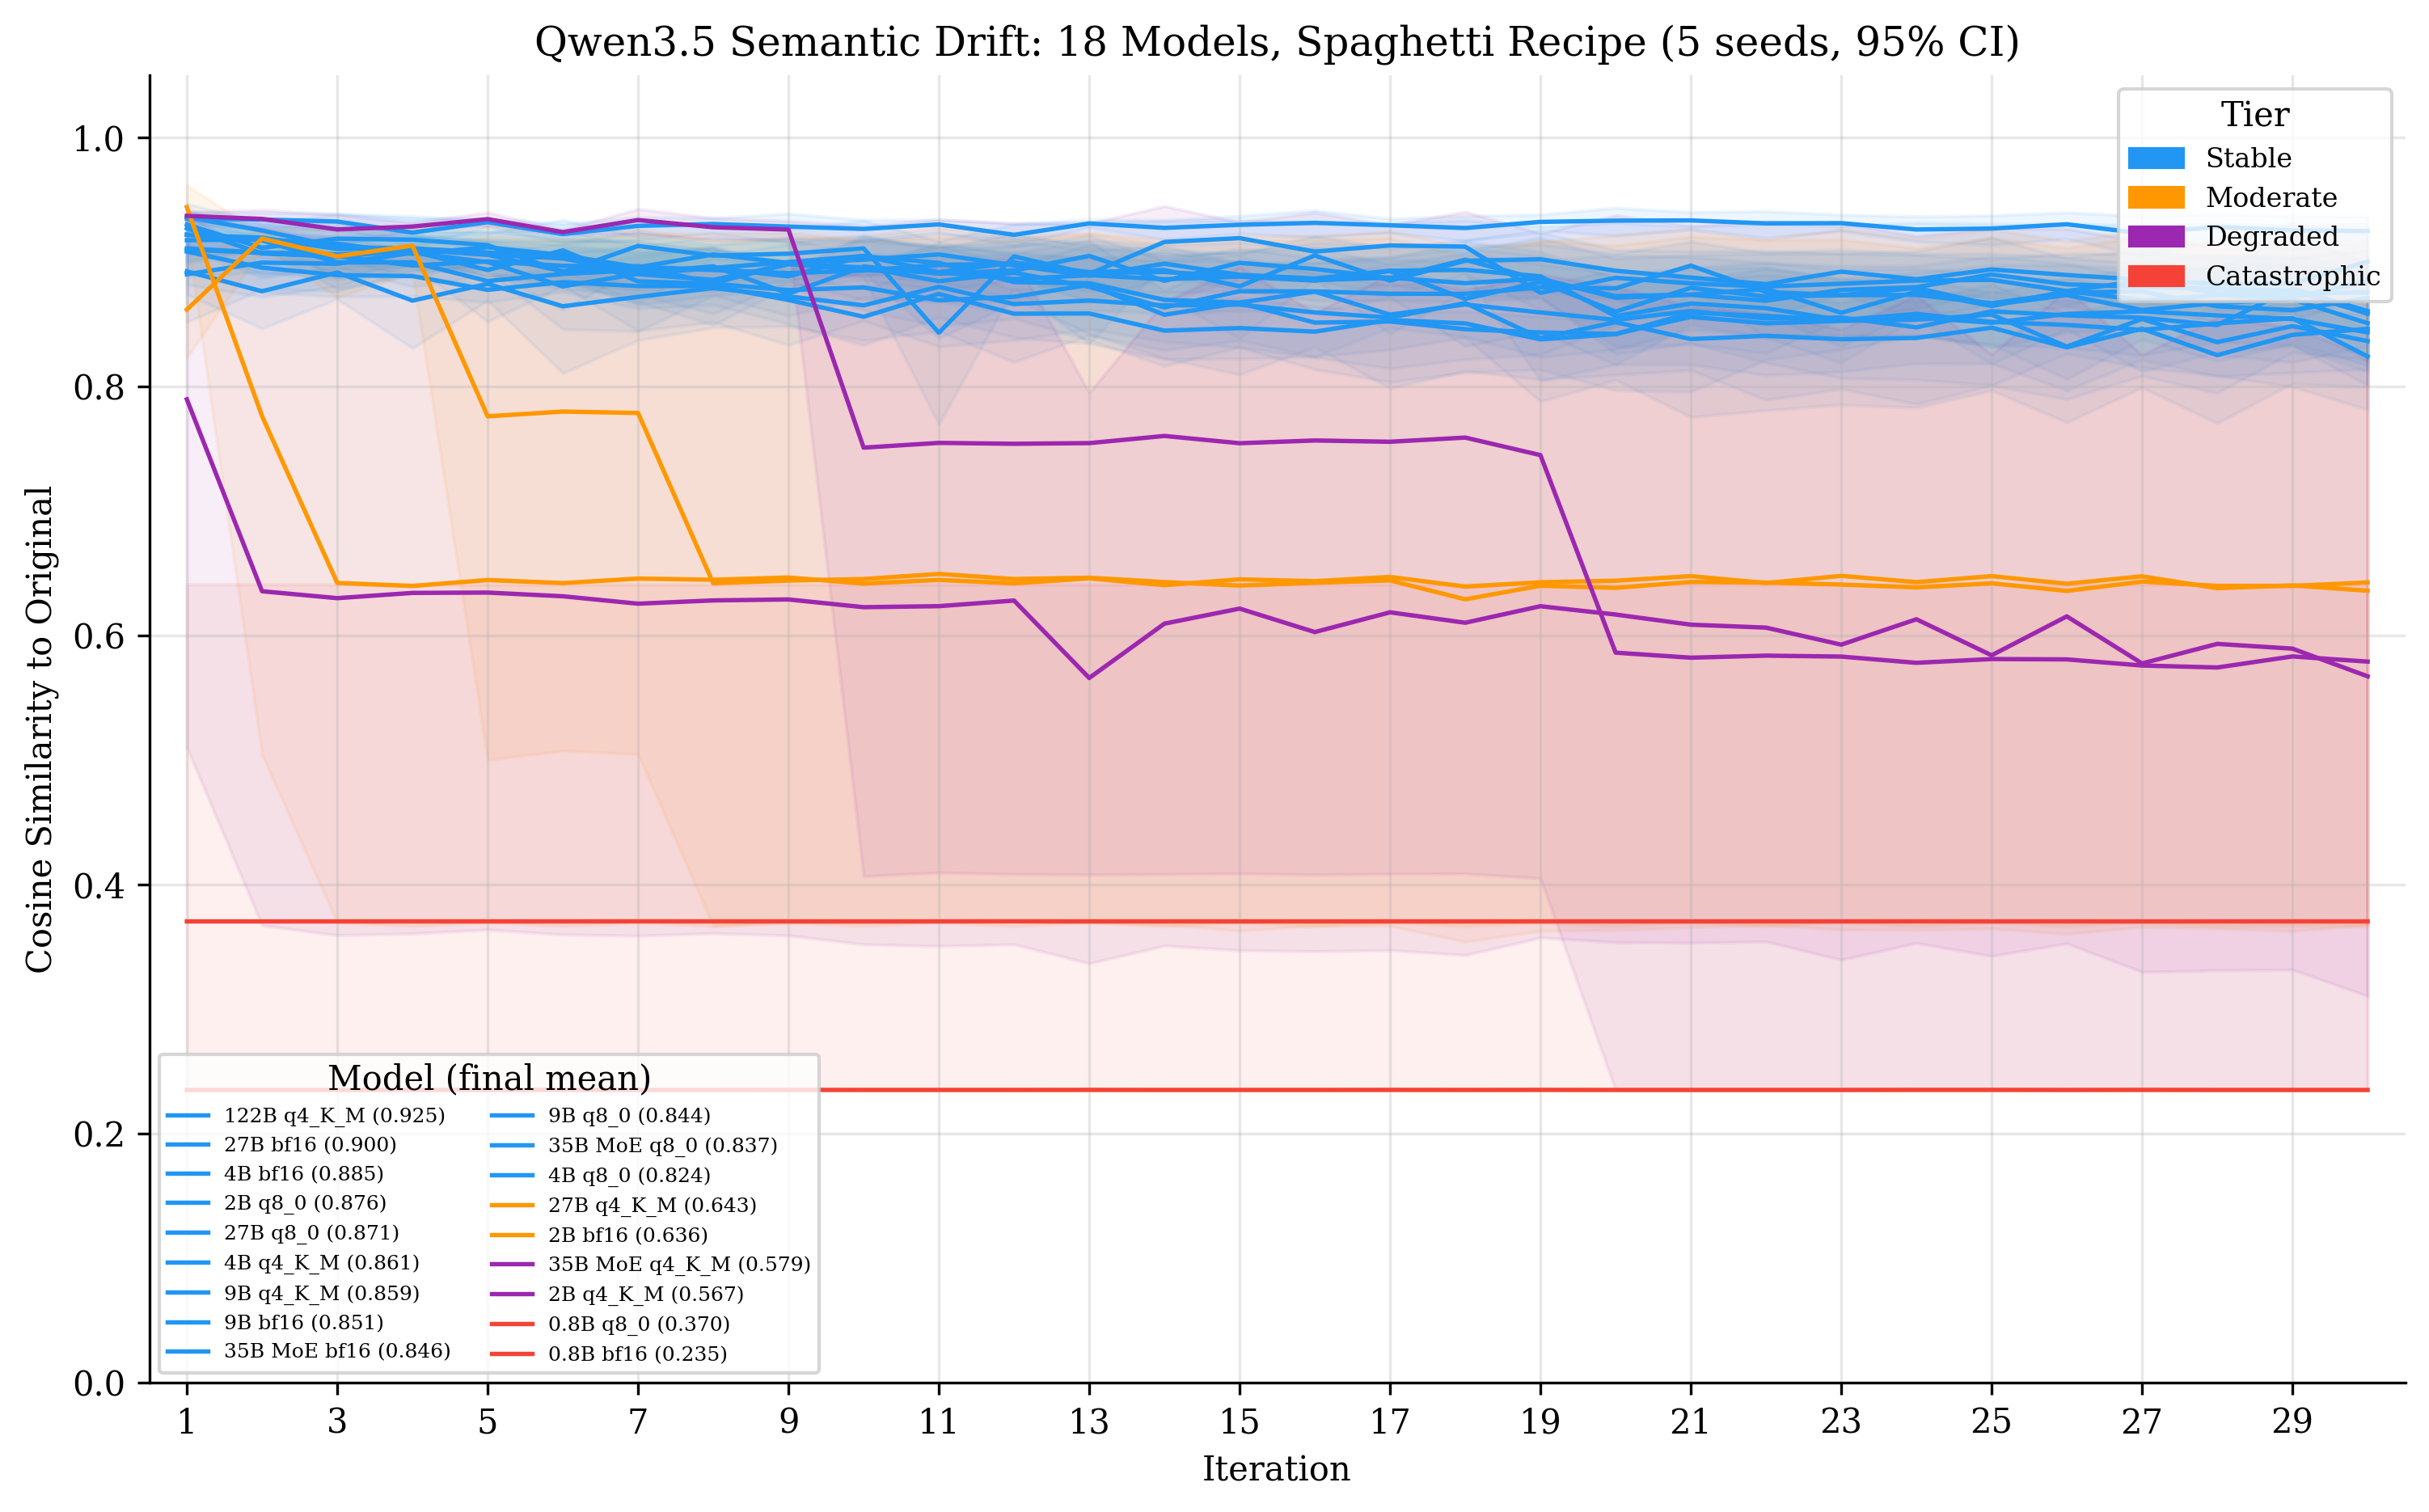
\includegraphics[width=\textwidth]{../results/qwen35_paper_figures/fig1_size_quant_lines.png}
\caption{Semantic drift across 18 Qwen3.5 GGUF models (spaghetti recipe,
  up to 5 completed chains per model, 95\% bootstrap CI bands). Models
  colored by stability tier; per-model $n$ is given in
  Table~\ref{tab:size_quant}.}
\label{fig:lines}
\end{figure}

\begin{table}[t]
\centering
\caption{Qwen3.5 drift by size and quantization. Mean final cosine
  similarity at iteration 30 over \emph{clean} chains only (chains with
  no empty, runaway-thinking generation), with 95\% bootstrap CI,
  sorted by clean spaghetti mean descending. $n_c$ is the number of
  clean 30-iteration chains behind each mean; ``RA'' is the
  runaway-thinking rate, i.e.\ the fraction of completed chains that
  contained at least one empty generation (runaway chains are excluded
  from the means). All-chain means are reported in the supplementary
  \texttt{all\_stats.json}.}
\label{tab:size_quant}
\footnotesize
\resizebox{\textwidth}{!}{%
\begin{tabular}{llcccccccl}
\toprule
Size & Quant & \multicolumn{4}{c}{Spaghetti} & \multicolumn{3}{c}{Lasagna} & Tier \\
\cmidrule(lr){3-6}\cmidrule(lr){7-9}
 & & Mean & 95\% CI & $n_c$ & RA & Mean & $n_c$ & RA & \\
\midrule
122B & q4\_K\_M & 0.925 & [0.915, 0.937] & 5 & 0.00 (0/5) & 0.864 & 5 & 0.00 (0/5) & Stable \\
35B MoE & q4\_K\_M & 0.923 & [0.920, 0.927] & 2 & 0.50 (2/4) & 0.812 & 5 & 0.00 (0/5) & Stable \\
27B & q4\_K\_M & 0.914 & [0.898, 0.929] & 3 & 0.40 (2/5) & 0.829 & 5 & 0.00 (0/5) & Stable \\
0.8B & q8\_0 & 0.912 & [0.912, 0.912] & 1 & 0.80 (4/5) & --- & 0 & 1.00 (5/5) & Stable \\
2B & bf16 & 0.903 & [0.892, 0.926] & 3 & 0.40 (2/5) & 0.760 & 2 & 0.60 (3/5) & Stable \\
27B & bf16 & 0.900 & [0.886, 0.914] & 5 & 0.00 (0/5) & 0.855 & 5 & 0.00 (0/5) & Stable \\
4B & bf16 & 0.885 & [0.873, 0.899] & 5 & 0.00 (0/5) & 0.741 & 5 & 0.00 (0/5) & Stable \\
2B & q8\_0 & 0.876 & [0.814, 0.931] & 5 & 0.00 (0/5) & 0.846 & 1 & 0.80 (4/5) & Stable \\
27B & q8\_0 & 0.871 & [0.833, 0.910] & 5 & 0.00 (0/5) & 0.839 & 5 & 0.00 (0/5) & Stable \\
4B & q4\_K\_M & 0.861 & [0.819, 0.899] & 5 & 0.00 (0/5) & 0.823 & 5 & 0.00 (0/5) & Stable \\
9B & q4\_K\_M & 0.859 & [0.820, 0.892] & 5 & 0.00 (0/5) & 0.830 & 5 & 0.00 (0/5) & Stable \\
9B & bf16 & 0.851 & [0.811, 0.893] & 5 & 0.00 (0/5) & 0.815 & 5 & 0.00 (0/5) & Stable \\
35B MoE & bf16 & 0.846 & [0.798, 0.887] & 5 & 0.00 (0/5) & 0.797 & 5 & 0.00 (0/5) & Stable \\
9B & q8\_0 & 0.844 & [0.783, 0.893] & 5 & 0.00 (0/5) & 0.795 & 5 & 0.00 (0/5) & Stable \\
35B MoE & q8\_0 & 0.837 & [0.815, 0.858] & 5 & 0.00 (0/5) & 0.803 & 5 & 0.00 (0/5) & Stable \\
4B & q8\_0 & 0.824 & [0.801, 0.846] & 5 & 0.00 (0/5) & 0.788 & 5 & 0.00 (0/5) & Stable \\
\midrule
2B & q4\_K\_M & 0.789 & [0.612, 0.889] & 3 & 0.40 (2/5) & 0.772 & 4 & 0.20 (1/5) & Moderate \\
\midrule
0.8B & bf16 & --- & --- & 0 & 1.00 (5/5) & --- & 0 & 1.00 (5/5) & Catastrophic \\
\bottomrule
\end{tabular}}
\end{table}


\paragraph{Stability threshold at 4B.}
Every model at or above 4B parameters reaches a mean final similarity of
at least 0.82 \emph{except} where whole chains collapse to the
empty-output floor of 0.235 (27B Q4\_K\_M, 0.643; 35B MoE Q4\_K\_M,
0.579); below 4B, no configuration is reliable. The 0.8B models are the
most fragile: BF16 sits at 0.235 in every chain (the embedding floor),
while Q8\_0 averages 0.370 with extreme seed variance (CI:
0.235--0.641). Many of these
low-similarity scores result from the model returning \emph{empty}
output strings---the API returns a successful response with no content.
The most likely explanation is that the model's internal thinking process
(Qwen3.5 models use a think-before-responding architecture) consumes
the entire generation budget on reasoning tokens, leaving nothing for
the final answer. This failure mode is consistent across seeds and
becomes more frequent as chain inputs degrade through drift. The 27B
models also exhibit sporadic empty outputs, particularly under Q4\_K\_M
quantization. These results suggest a minimum capacity threshold below
which models cannot reliably maintain semantic content through iterated
paraphrasing.

\paragraph{Non-monotonic quantization.}
Quantization effects are not monotonic. For the 4B dense model, BF16
(0.885) leads, followed by Q4\_K\_M (0.861) and Q8\_0 (0.824). The 2B
model shows Q8\_0 (0.876) far ahead of BF16 (0.636) and Q4\_K\_M
(0.567), a reversal of more than 0.30 between the two higher-precision
formats. For the 35B MoE, BF16 (0.846) and Q8\_0 (0.837) are close
together while Q4\_K\_M falls to 0.579 ($n=4$); for the 27B dense model
BF16 (0.900) and Q8\_0 (0.871) likewise sit well above Q4\_K\_M
(0.643). In both of the latter cases the gap is driven by whole chains
collapsing to the empty-output floor rather than by gradual degradation,
and the corresponding confidence intervals are correspondingly wide
(35B MoE Q4\_K\_M: [0.235, 0.923]). These reversals confirm Paper~1's
finding that higher precision does not guarantee less drift, but they
also show that at 4-bit the dominant risk is a discrete generation
failure rather than a smooth loss of fidelity.

\paragraph{MoE architectures.}
The 122B MoE achieves the family's best score (0.925, CI [0.915, 0.937])
and is the only model whose interval excludes 0.90 from below. At
comparable parameter counts the 35B MoE (0.579--0.846) does not beat the
27B dense models (0.643--0.900): on this data the sparse-activation
advantage suggested by Paper~1 is not reproduced within the Qwen3.5
family once empty-output failures are counted.

\paragraph{Statistical tests.}
Kruskal--Wallis over the four occupied tiers confirms significant
differences ($H = 18.19$, $p = 4.0 \times 10^{-4}$). Cohen's $d$ between
the Stable and Catastrophic tiers is 6.18 and between Stable and Moderate
1.67. As in Paper~1, the test treats the individual seed-chains as
observations even though chains from the same model are not independent
of one another, so it should be read as descriptive rather than
inferential.

Figure~\ref{fig:heatmap} presents the size $\times$ quantization heatmap.

\begin{figure}[t]
\centering
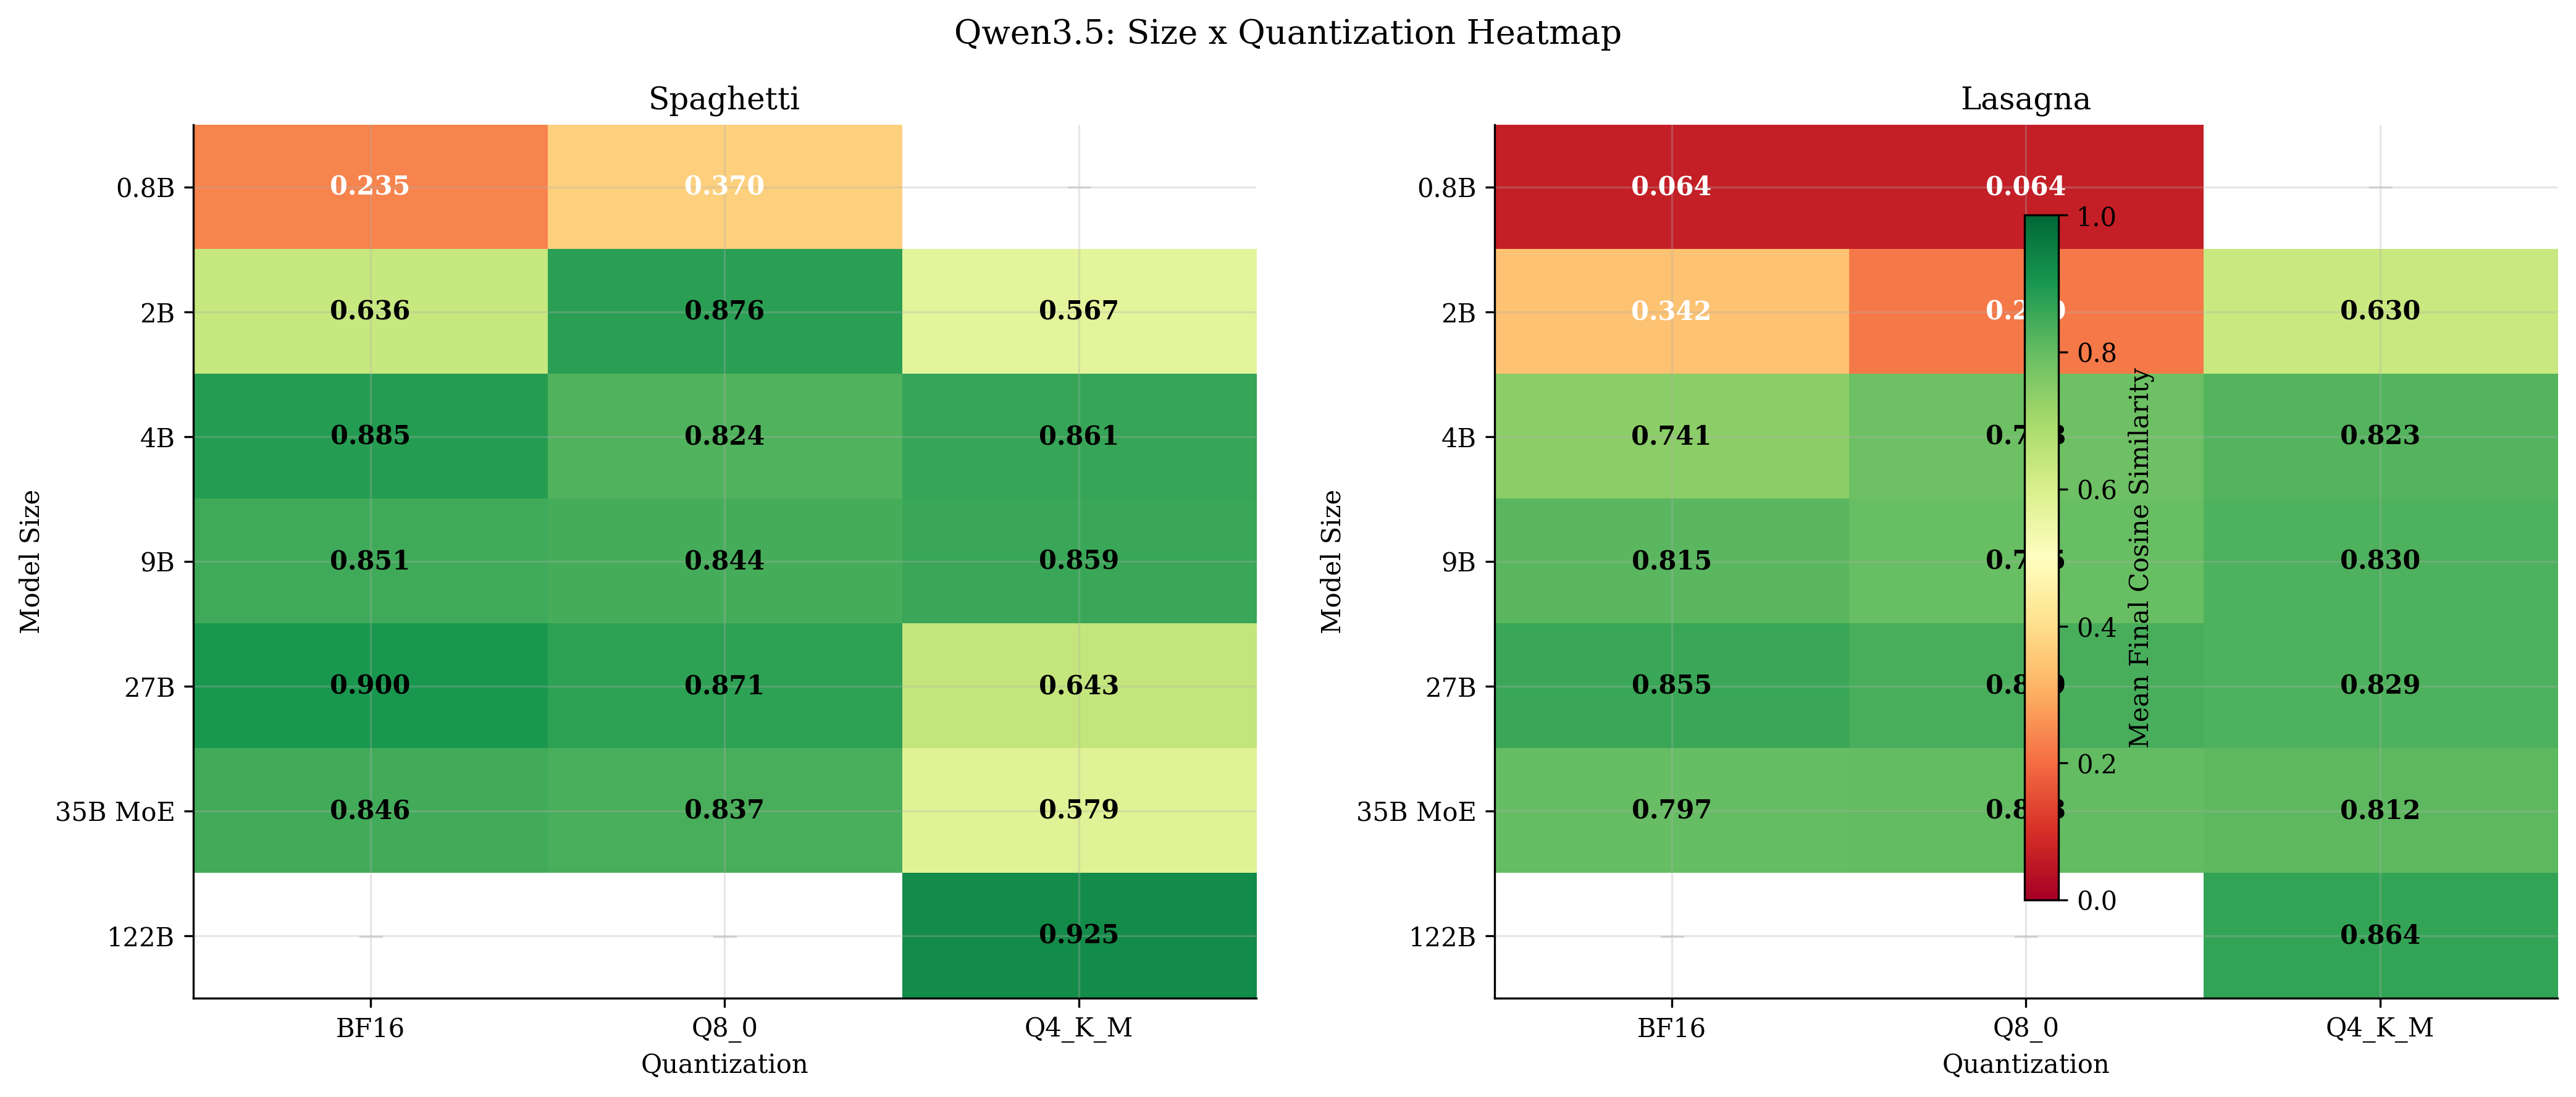
\includegraphics[width=\textwidth]{../results/qwen35_paper_figures/fig3_quant_heatmap.png}
\caption{Mean final similarity by model size and quantization level.
  Left: spaghetti recipe. Right: lasagna recipe.
  Note that 0.8B Q4\_K\_M does not exist for Qwen3.5.}
\label{fig:heatmap}
\end{figure}

\clearpage

\subsection{RQ2: GGUF vs.\ AWQ vs.\ NVFP4 vs.\ GPTQ-Int4 Quantization}
\label{sec:rq2}

Figure~\ref{fig:awq} compares the 35B MoE model under four quantization
methods: GGUF Q4\_K\_M (Ollama), AWQ 4-bit (vLLM), NVFP4 4-bit (sglang),
and GPTQ-Int4 (vLLM). All four are 4-bit quantizations of the same
underlying Qwen3.5-35B-A3B architecture, differing only in quantization
algorithm and serving backend.

\begin{figure}[t]
\centering
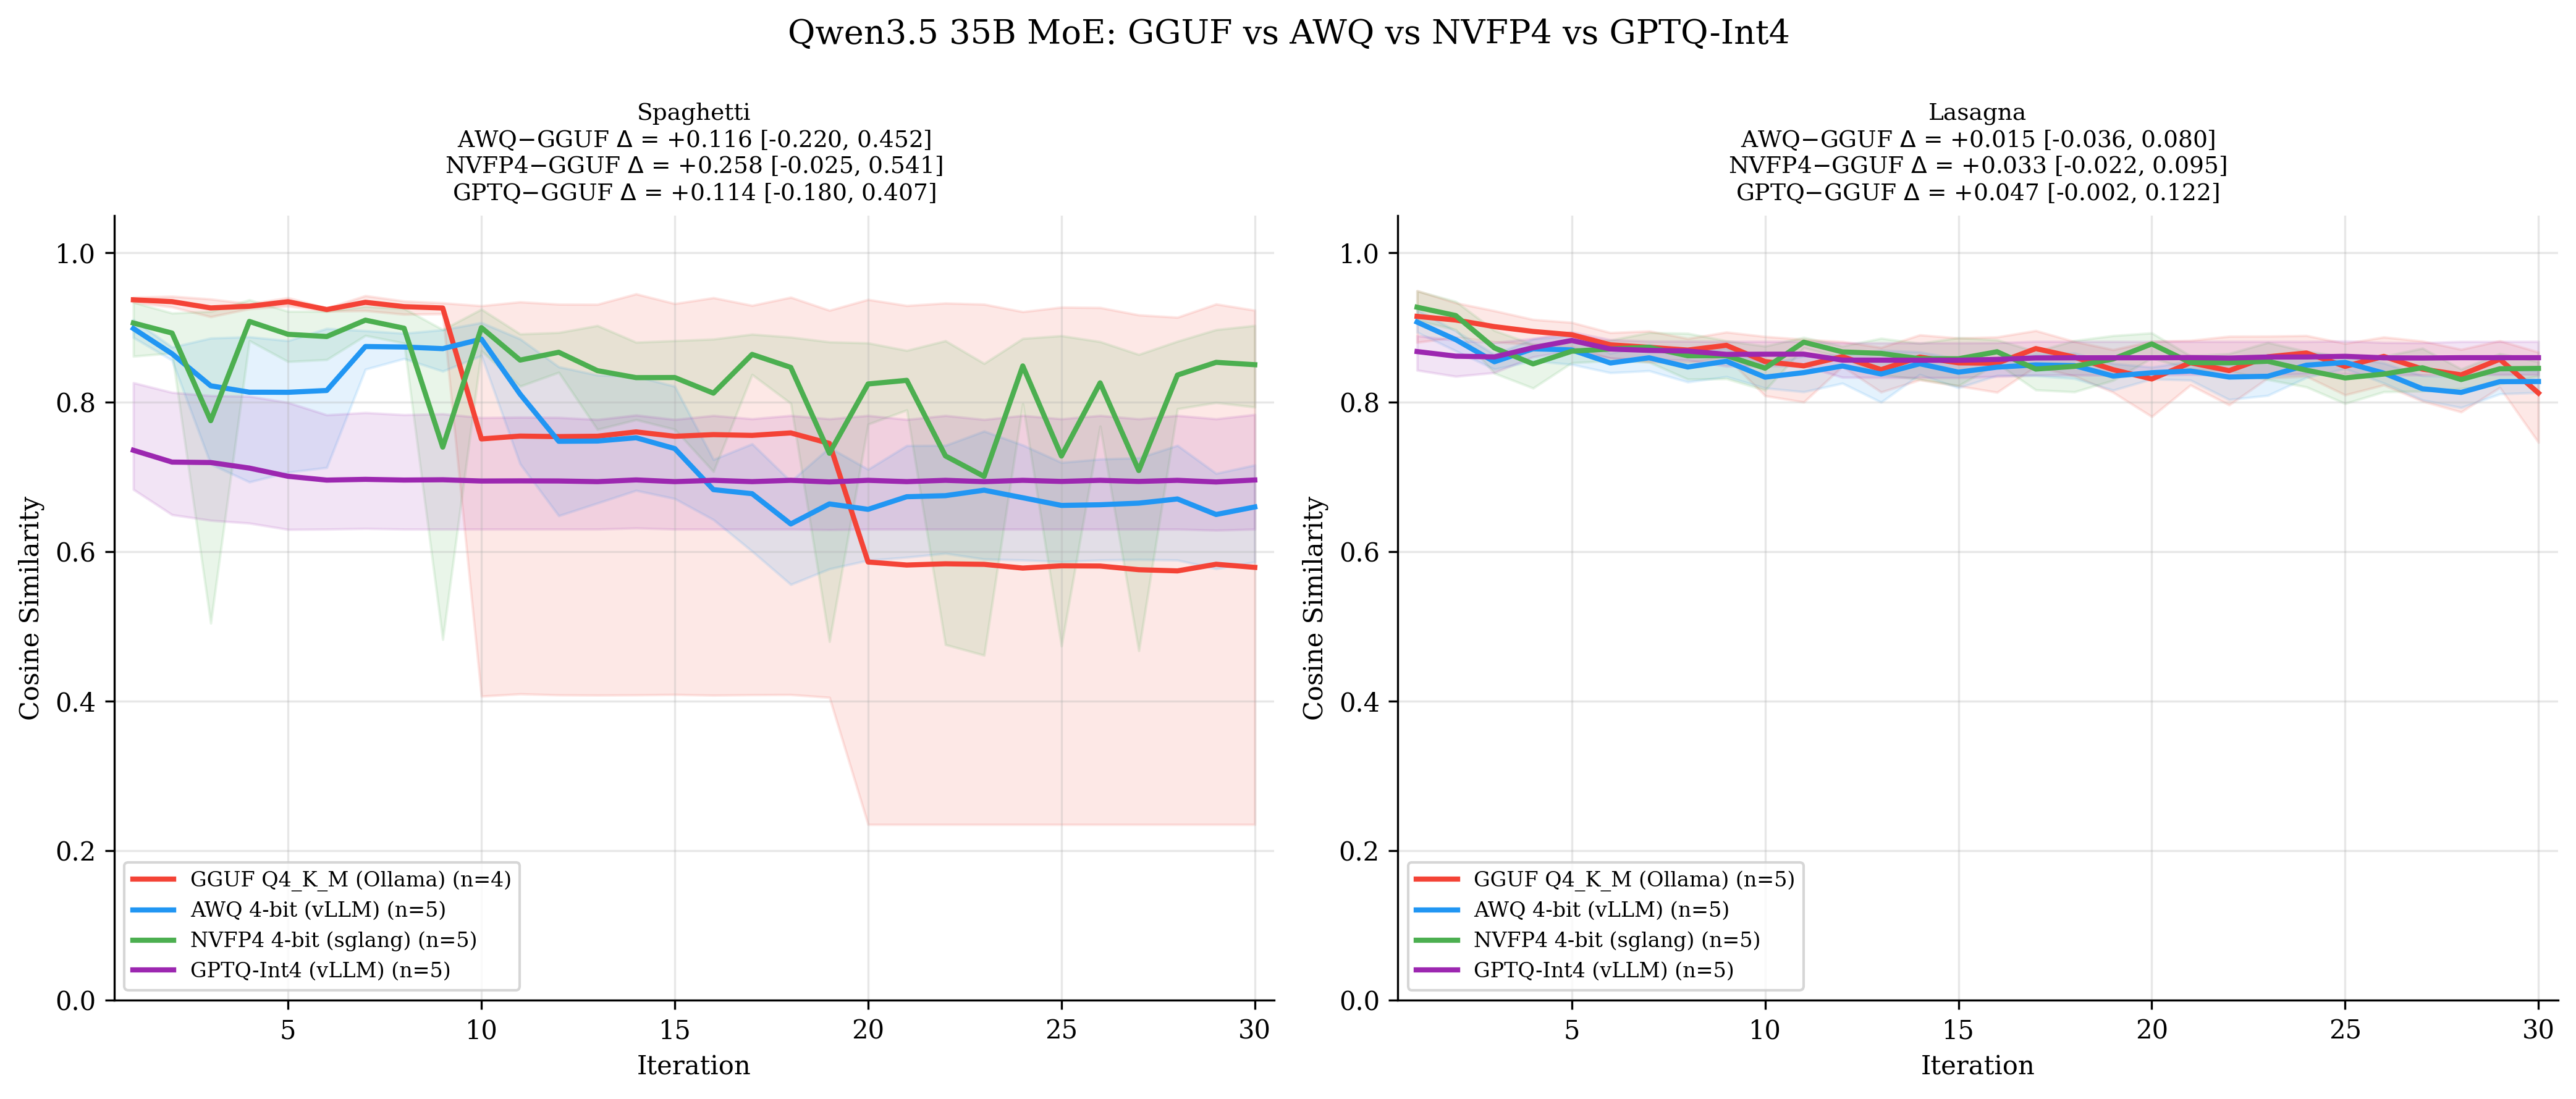
\includegraphics[width=\textwidth]{../results/qwen35_paper_figures/fig4_gguf_vs_awq.png}
\caption{Four quantization methods for the 35B MoE model: GGUF Q4\_K\_M
  (Ollama), AWQ 4-bit (vLLM), NVFP4 4-bit (sglang), and GPTQ-Int4 (vLLM).
  Left: spaghetti. Right: lasagna. Panel titles give the seed-matched
  paired delta against GGUF with its bootstrap 95\% CI; $n$ per arm is
  shown in the legend.}
\label{fig:awq}
\end{figure}

%% FABLE-REWRITE: the two paragraphs below are stale. Rewrite by hand from
%% results/qwen35_paper_figures/summary_for_text.md (section 2), which now
%% carries a four-way GGUF / AWQ / NVFP4 / GPTQ-Int4 comparison with paired
%% seed-matched deltas and bootstrap CIs.
On the spaghetti recipe, GGUF Q4\_K\_M achieves 0.920 while AWQ drops to
0.660---a large delta of $-$0.260. This suggests that the AWQ quantization
method, despite being optimized for inference throughput, may introduce
different error patterns than GGUF's round-to-nearest approach. The
difference is recipe-dependent: on the more complex lasagna prompt, AWQ
achieves 0.828 while GGUF performance varies by quantization level.

NVFP4 (NVIDIA's FP4 format) and GPTQ-Int4 provide two further data
points, allowing us to distinguish between quantization algorithm effects
and serving backend effects.
%% FABLE-REWRITE ends here.

This finding extends Paper~1's observation that AWQ and GGUF produce
different drift dynamics for Qwen3-VL 30B, and suggests that the choice
of quantization \emph{method}---not just precision level---is a significant
factor in multi-agent pipeline reliability.

\subsection{RQ3: Temperature}
\label{sec:rq3}

Figure~\ref{fig:temp} shows temperature sensitivity across eight
configurations (4 Ollama GGUF, the 35B AWQ, NVFP4 and GPTQ-Int4 variants,
the 9B AWQ variant, and the Nemotron control).

\begin{figure}[t]
\centering
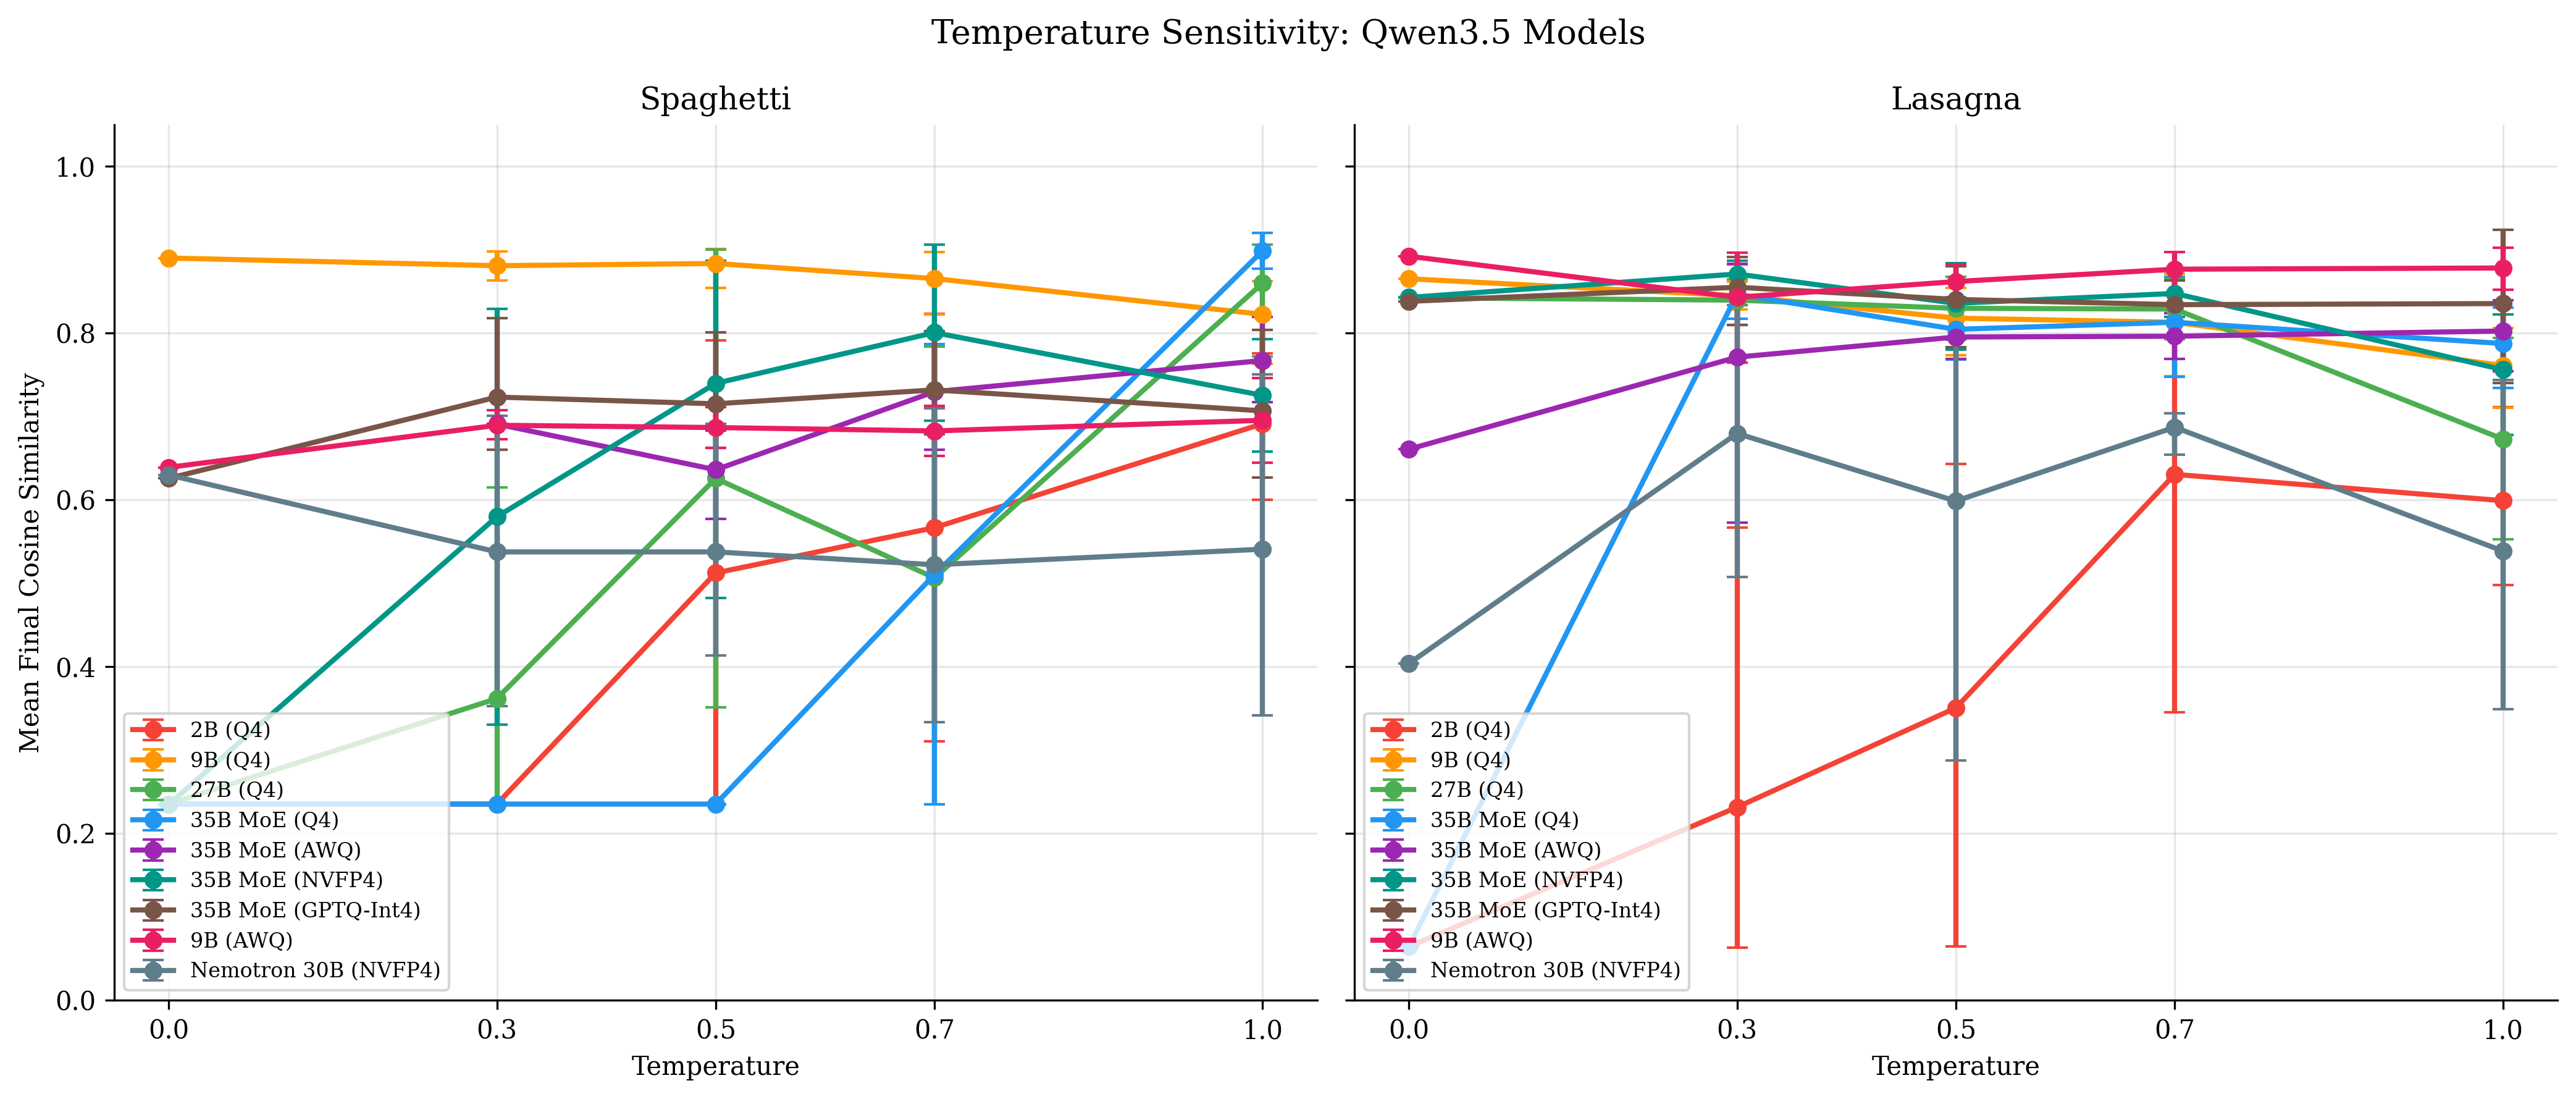
\includegraphics[width=\textwidth]{../results/qwen35_paper_figures/fig5_temperature.png}
\caption{Temperature sensitivity across Qwen3.5 models. Left: spaghetti.
  Right: lasagna.}
\label{fig:temp}
\end{figure}

\paragraph{Size-dependent temperature sensitivity.}
The 9B GGUF model shows remarkable temperature insensitivity: final
similarity ranges only 0.823--0.890 across $T \in [0.0, 1.0]$ on
spaghetti. In contrast, the 2B model shows \emph{inverted} temperature
sensitivity on spaghetti: $T=0.0$ and $T=0.3$ both sit at the
empty-output floor of 0.235, and similarity then rises monotonically with
temperature (0.512 at $T=0.5$, 0.567 at $T=0.7$, 0.691 at $T=1.0$). The
same inversion appears for the 35B MoE GGUF model, which is pinned at
0.235 for $T \leq 0.5$ and reaches 0.899 at $T=1.0$. This
suggests that low-temperature deterministic sampling can trap small models
in repetitive attractor loops that the embedding model scores favorably,
while moderate temperatures disrupt this lock-in without providing enough
diversity to maintain content.

\paragraph{AWQ temperature profile.}
The 35B AWQ model shows a qualitatively different pattern: similarity
\emph{increases} with temperature on both recipes (spaghetti: 0.636 at
$T=0.5$ to 0.767 at $T=1.0$; lasagna: 0.661 at $T=0.0$ to 0.803 at
$T=1.0$; the AWQ $T=0.0$ spaghetti chain was among those lost to the
failed rerun). The 35B GPTQ-Int4 and 9B AWQ variants are by contrast
nearly flat across the whole temperature range (GPTQ spaghetti
0.626--0.732; 9B~AWQ spaghetti 0.639--0.696). This is the
opposite of the conventional expectation that higher temperature increases
randomness and thus drift. We hypothesize that the AWQ quantization
creates a restricted output distribution at low temperatures, and higher
temperature actually helps the model access more of its learned paraphrase
space.

\subsection{RQ4: System Prompts}
\label{sec:rq4}

We test whether Paper~1's system prompt findings generalize within the
Qwen3.5 family by running the same 20 system prompts across six Qwen3.5
configurations---9B and 27B GGUF (Ollama, Exp~4), 35B AWQ (Exp~3c), 35B
NVFP4 (Exp~3d), 35B GPTQ-Int4 (Exp~3e) and 9B AWQ (Exp~3f)---plus the
out-of-family Nemotron-3-Nano-30B control (Exp~3g). Each condition uses
up to 5 completed chains on both the spaghetti and lasagna recipes;
Table~\ref{tab:rq4_spread} summarizes the per-configuration spread,
best and worst prompt, and the pairwise Spearman rank correlations, and
Table~\ref{tab:sysprompt} gives the per-prompt means.

\begin{figure}[t]
\centering
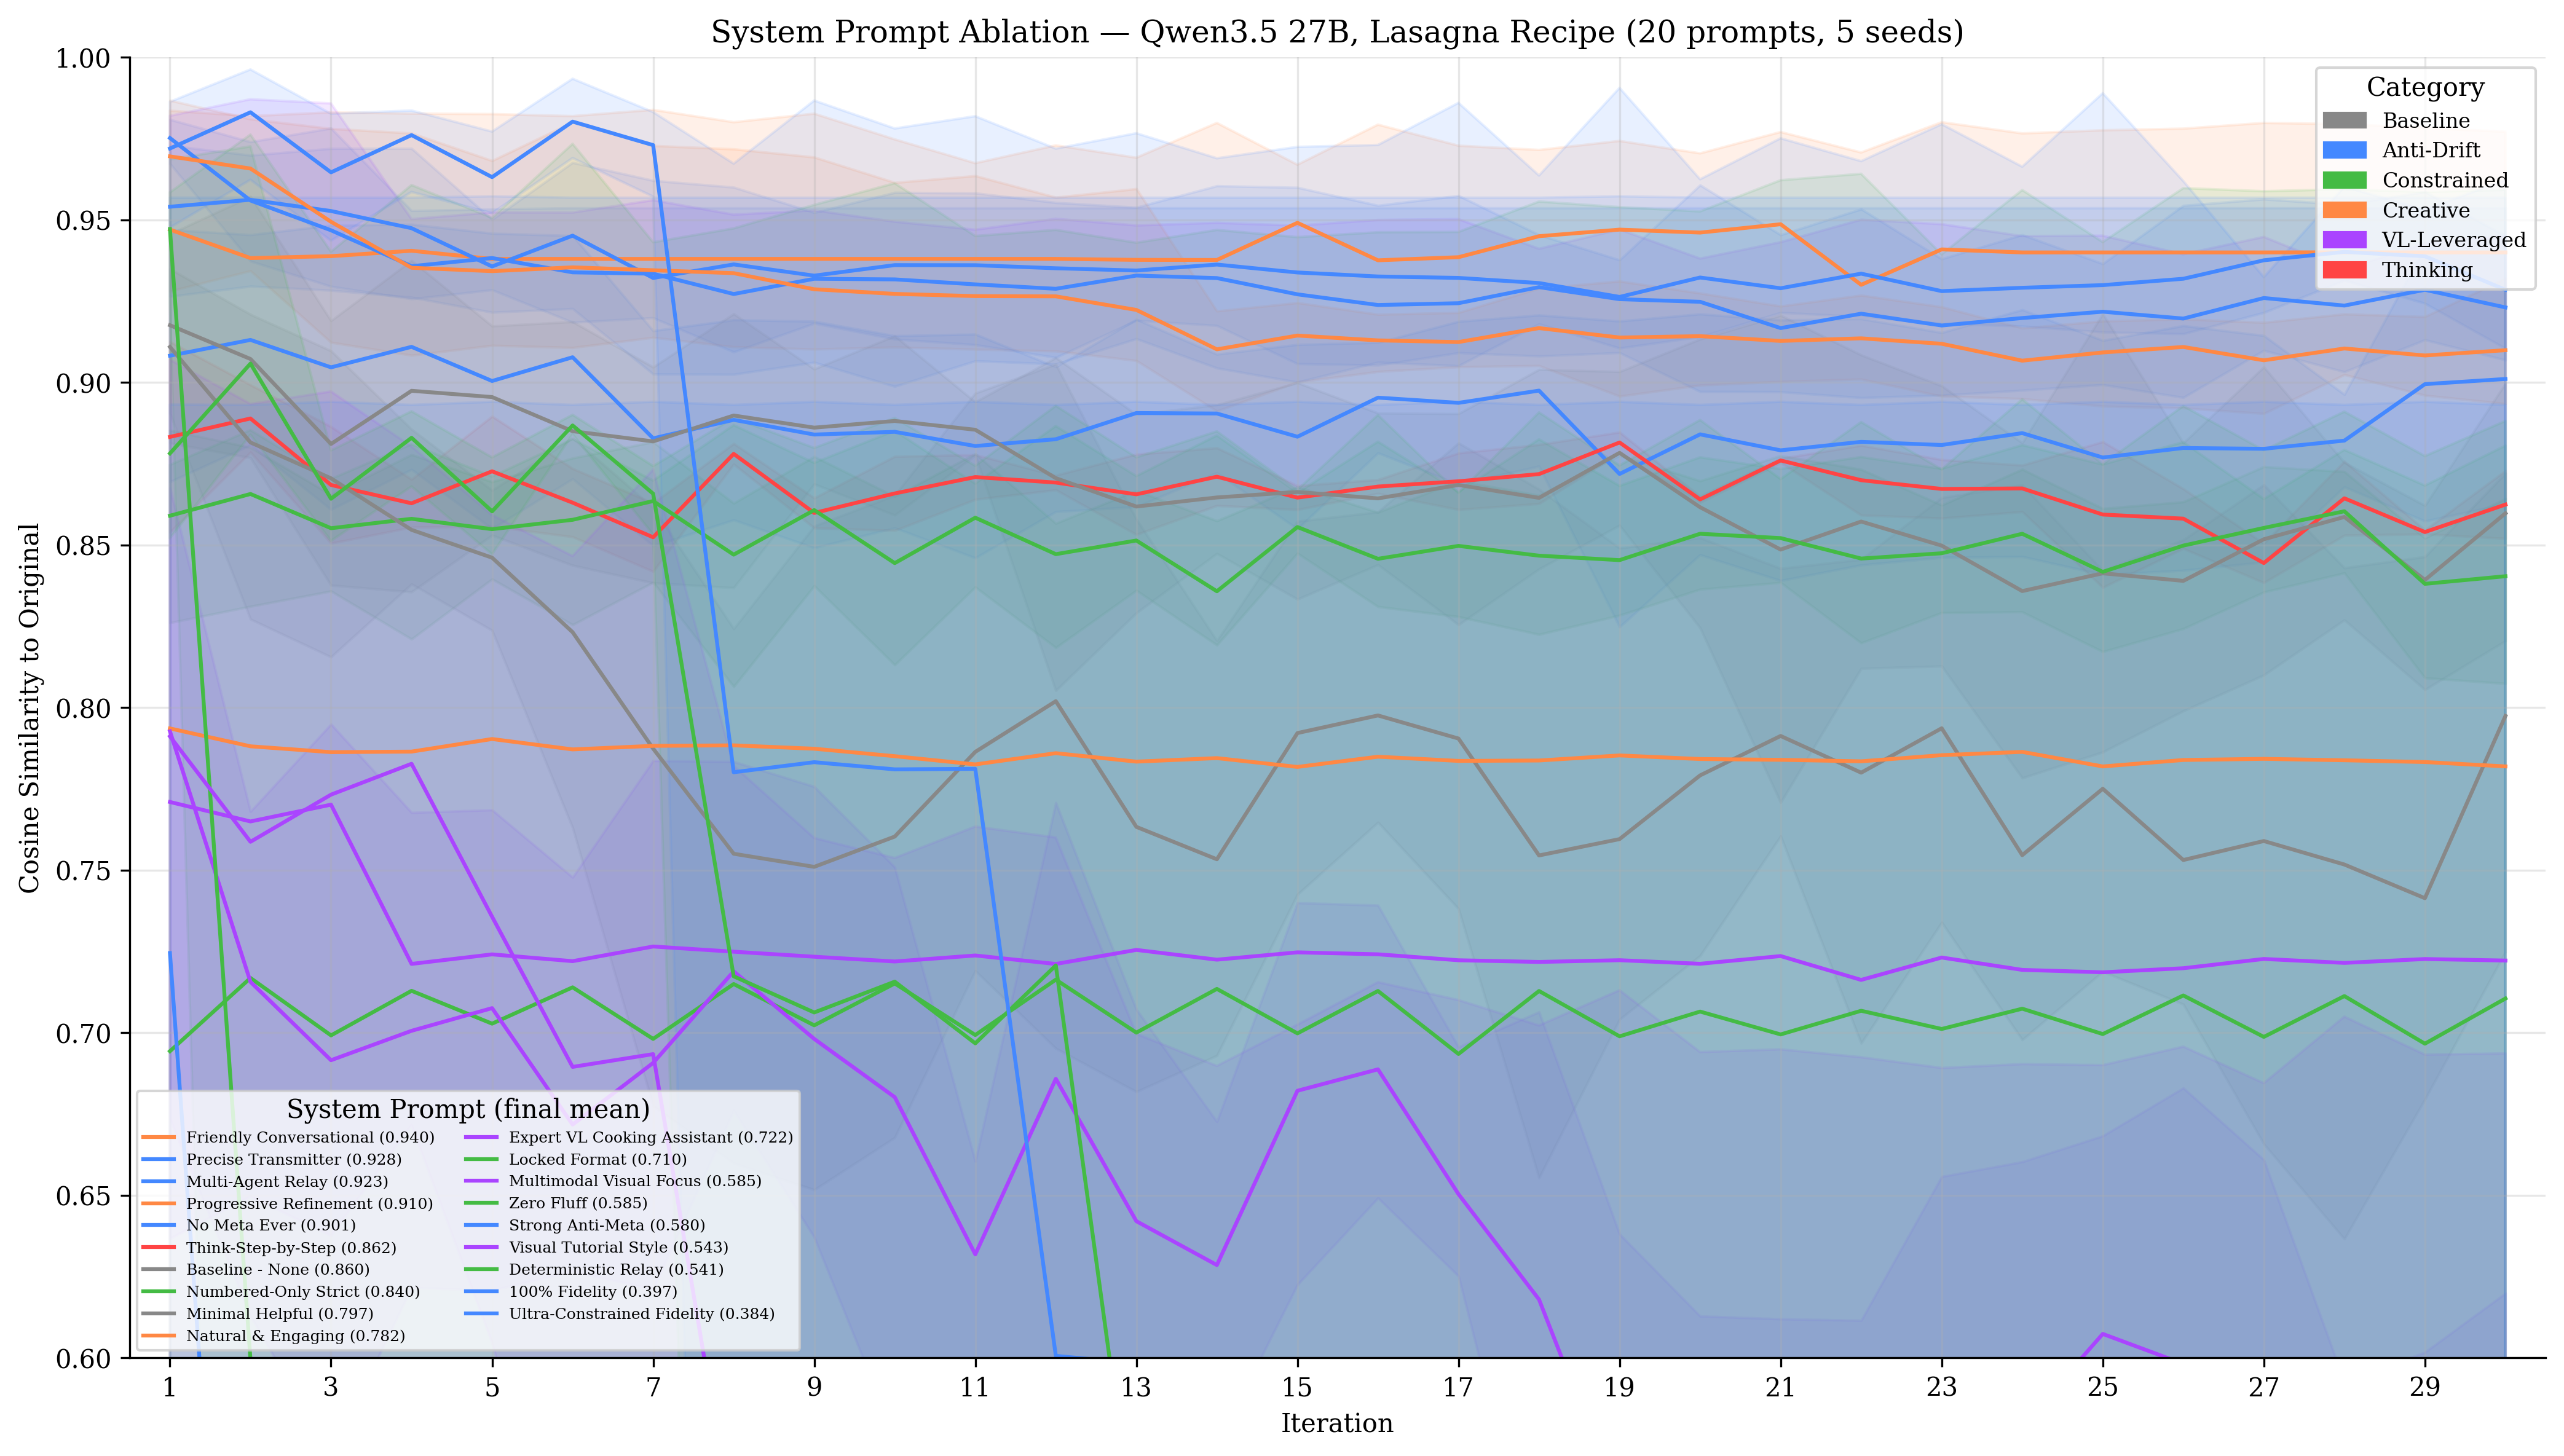
\includegraphics[width=\textwidth]{../results/qwen35_paper_figures/fig7_sysprompt_hero.png}
\caption{System prompt ablation on Qwen3.5 27B GGUF, lasagna recipe.
  20 prompts shown with mean $\pm$ min/max band over the completed chains
  for each prompt. Prompts 15--20 rest on fewer than 5 chains and
  ``Balanced Clarity'' on none (Section~\ref{sec:method}).}
\label{fig:syshero}
\end{figure}

\begin{figure}[t]
\centering
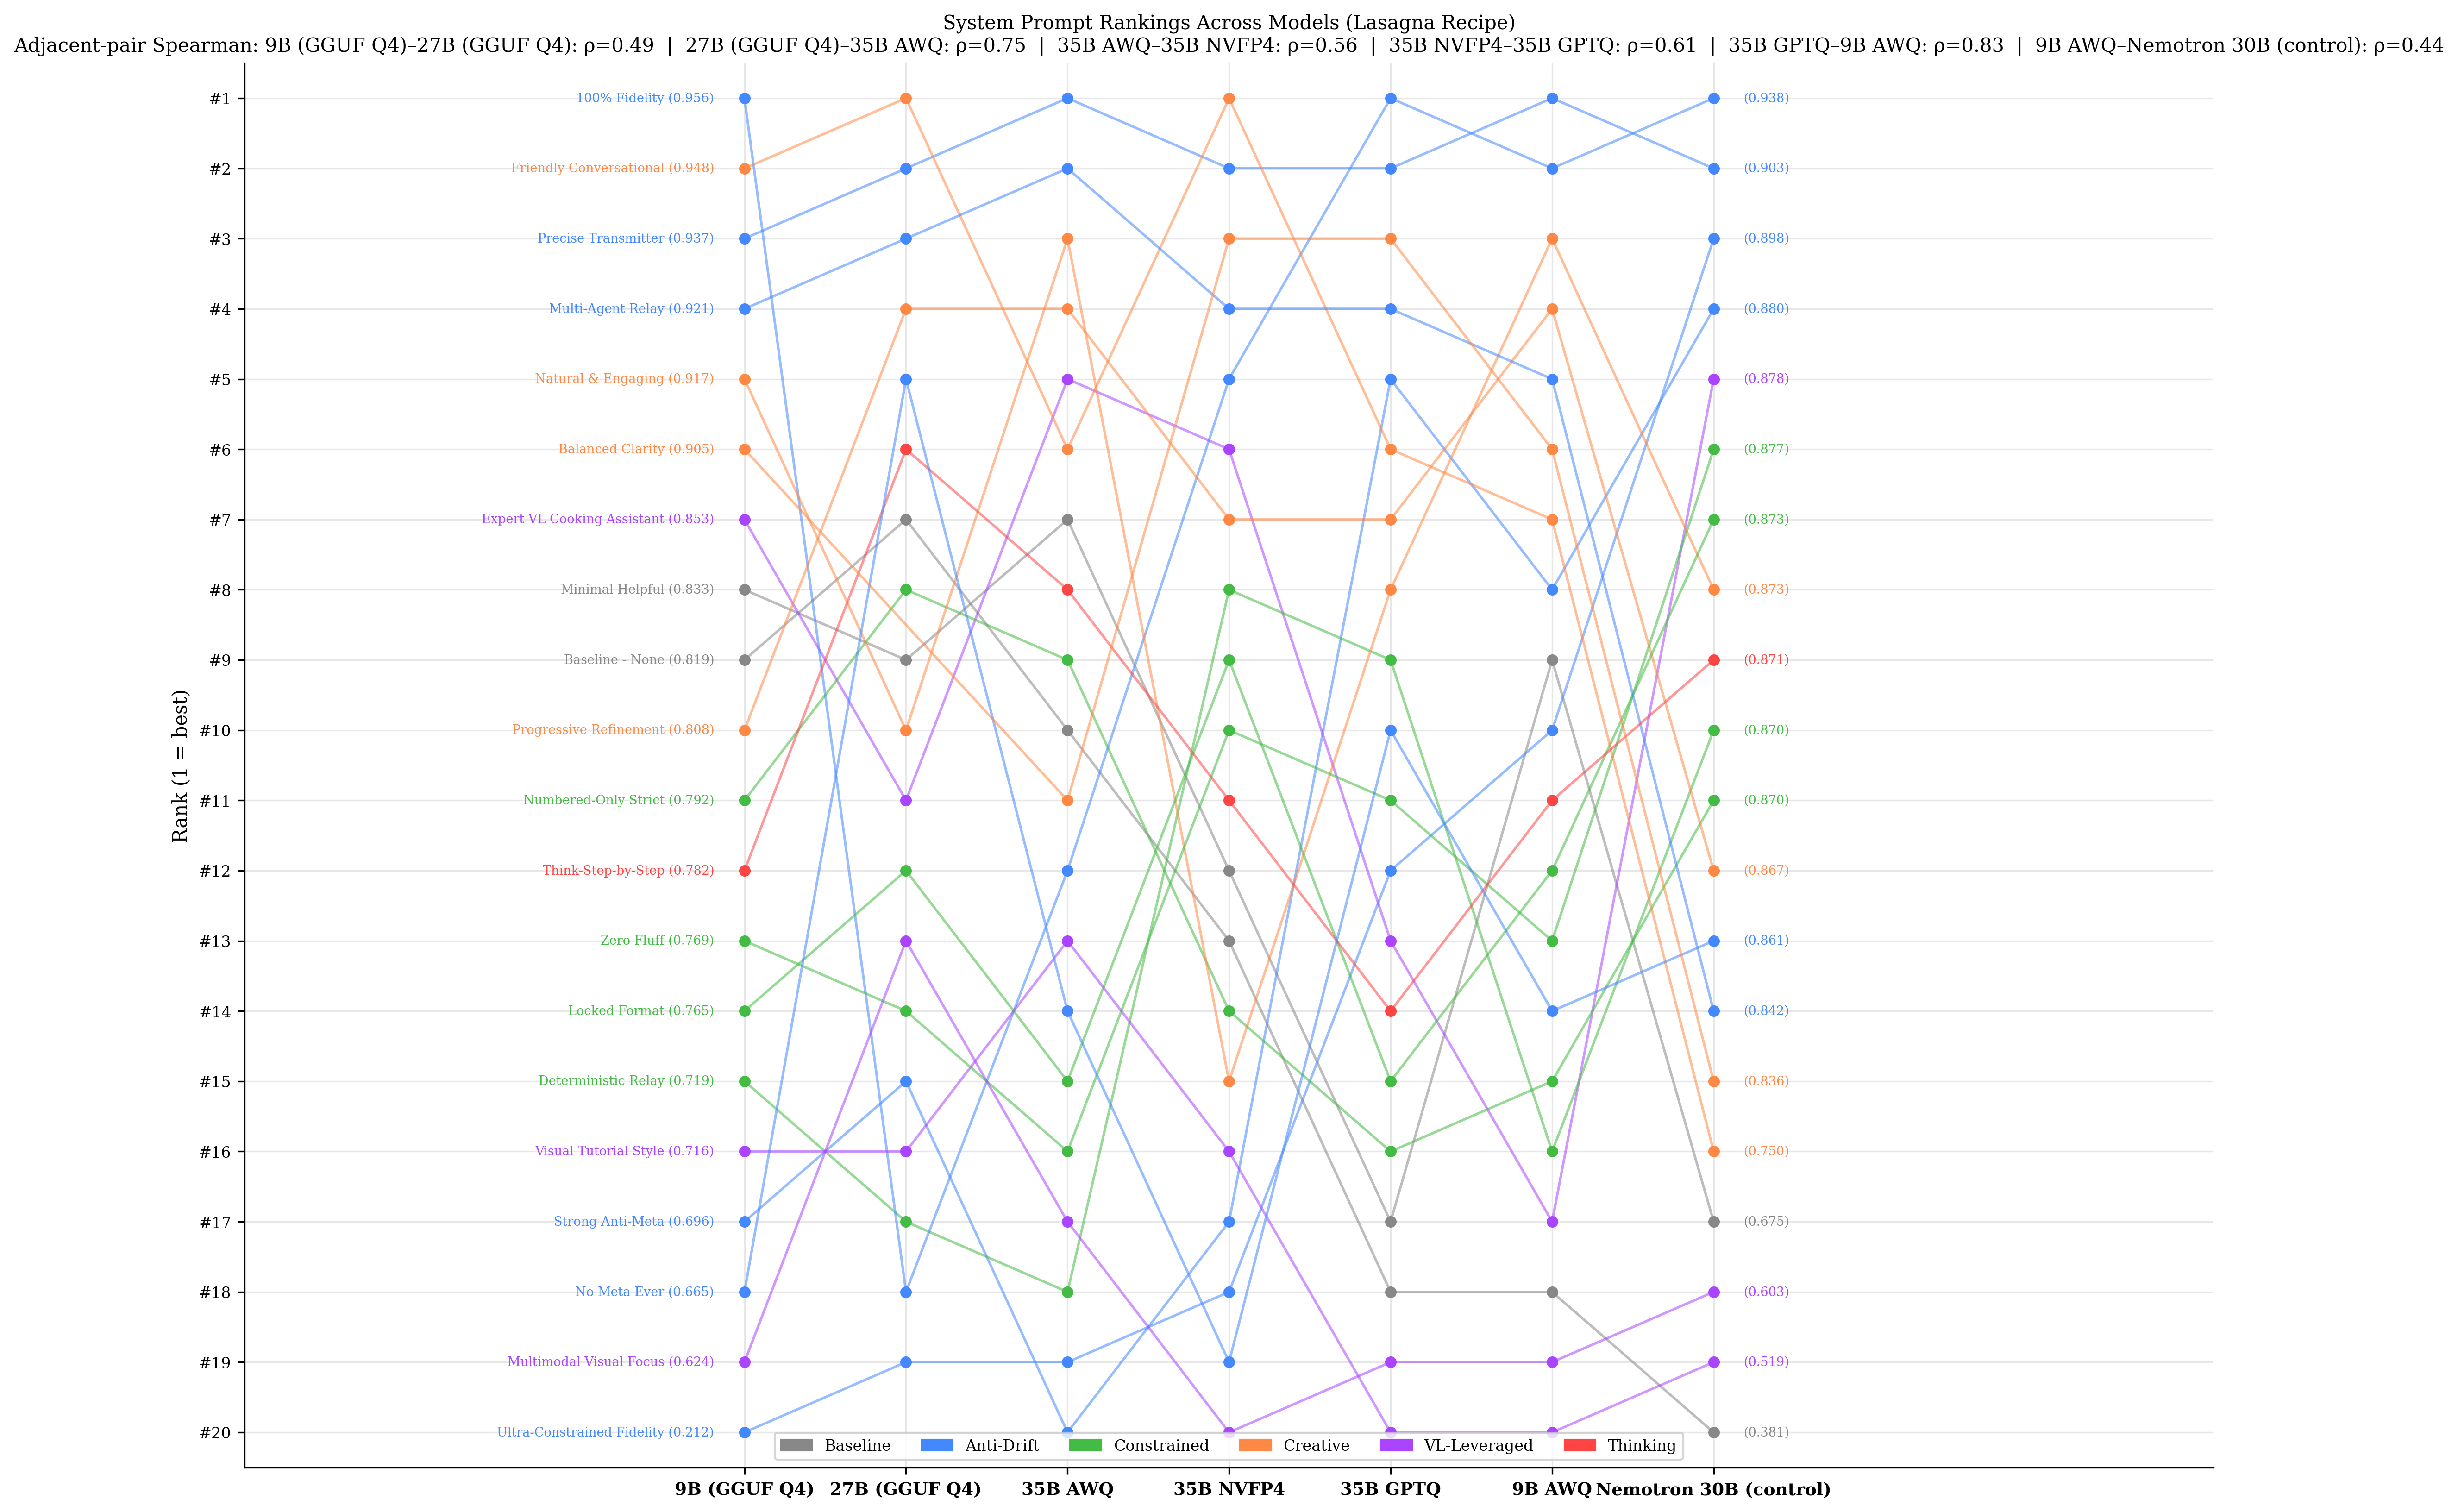
\includegraphics[width=\textwidth]{../results/qwen35_paper_figures/fig8_sysprompt_cross_model.png}
\caption{System prompt rankings across all six Qwen3.5 configurations and
  the Nemotron control (lasagna). Adjacent-column Spearman $\rho$ values
  are annotated; the full matrix with bootstrap CIs is in
  Table~\ref{tab:rq4_spread}.}
\label{fig:syscross}
\end{figure}

\begin{figure}[t]
\centering
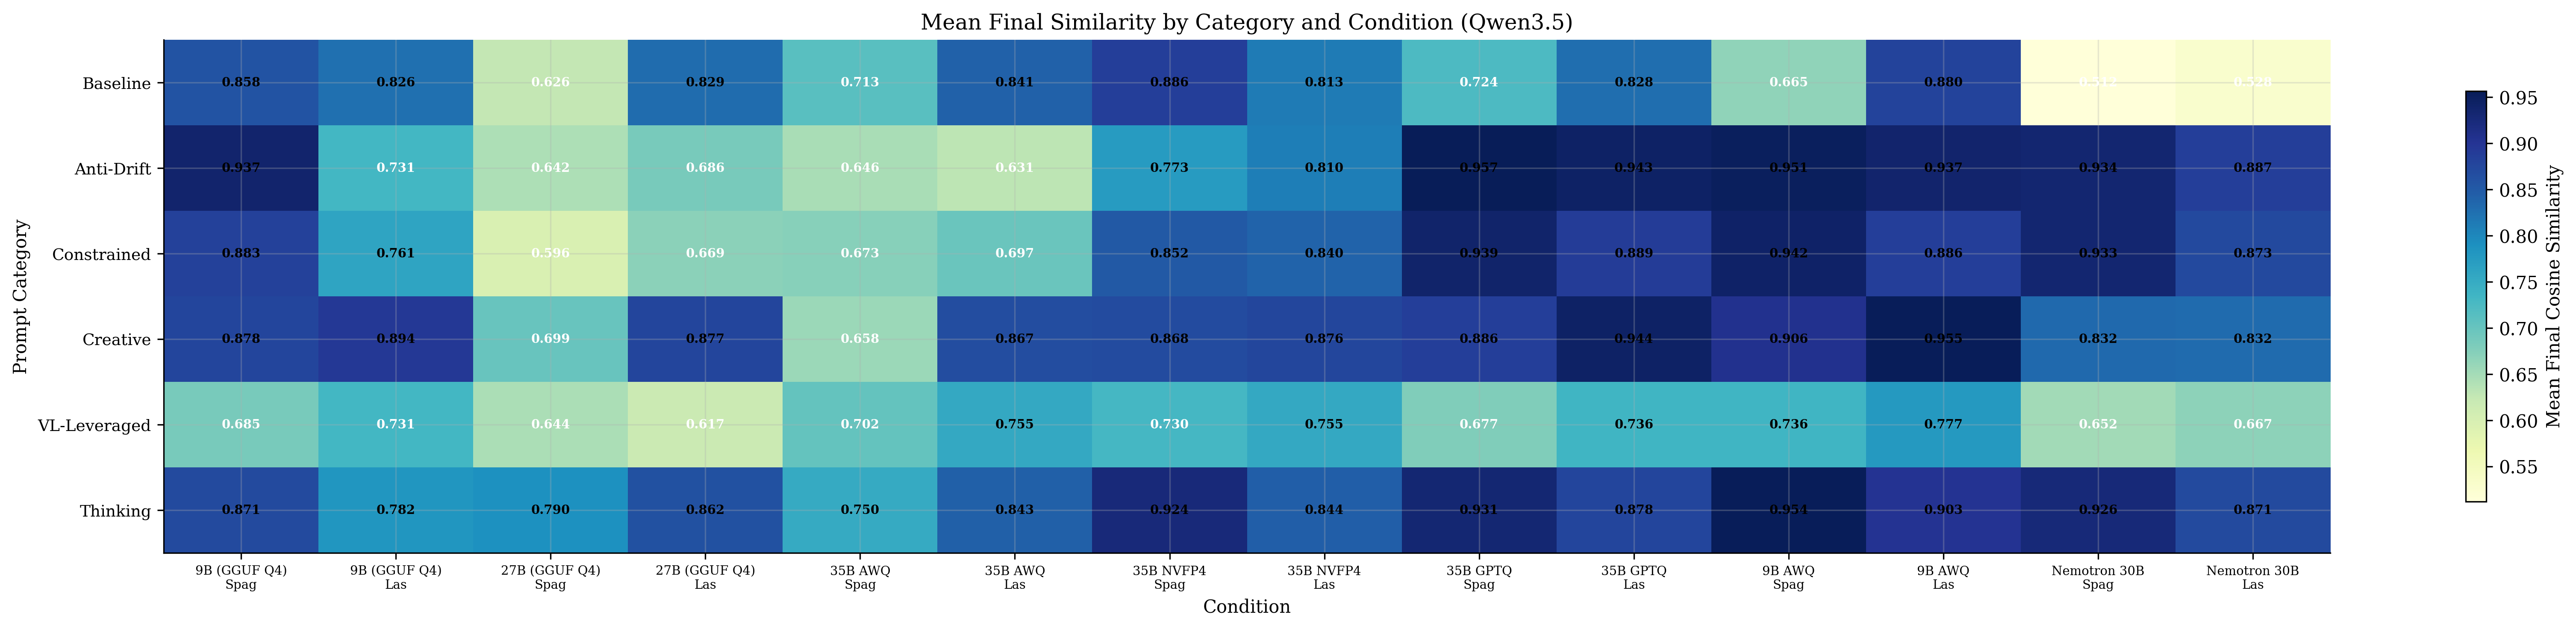
\includegraphics[width=0.9\textwidth]{../results/qwen35_paper_figures/fig9_category_heatmap.png}
\caption{Mean final similarity by prompt category and condition.}
\label{fig:catheat}
\end{figure}

\begin{table}[t]
\centering
\caption{RQ4 summary (lasagna recipe), computed over \emph{clean}
  chains only. Spread is the difference between the best- and
  worst-performing system prompt for that configuration;
  $n_{\min}$ is the smallest number of clean chains behind any
  prompt cell; ``RA'' is the configuration-wide runaway-thinking rate
  over all 20 prompts $\times$ 5 seeds.}
\label{tab:rq4_spread}
\small
\resizebox{\textwidth}{!}{%
\begin{tabular}{lccllcc}
\toprule
Configuration & Mean & Spread & Best prompt & Worst prompt & $n_{\min}$ & RA \\
\midrule
9B (GGUF Q4) & 0.822 & 0.332 & 100\% Fidelity (0.956) & Multimodal Visual Focus (0.624) & 1 & 0.05 (5/97) \\
27B (GGUF Q4) & 0.868 & 0.380 & Natural \& Engaging (0.965) & Multimodal Visual Focus (0.585) & 1 & 0.20 (16/81) \\
35B AWQ & 0.742 & 0.743 & Precise Transmitter (0.917) & Strong Anti-Meta (0.175) & 5 & 0.00 (0/100) \\
35B NVFP4 & 0.854 & 0.294 & Balanced Clarity (0.956) & Multimodal Visual Focus (0.663) & 2 & 0.30 (30/99) \\
35B GPTQ & 0.887 & 0.348 & 100\% Fidelity (0.981) & Visual Tutorial Style (0.633) & 4 & 0.00 (0/99) \\
9B AWQ & 0.899 & 0.300 & Precise Transmitter (0.972) & Visual Tutorial Style (0.672) & 4 & 0.00 (0/99) \\
Nemotron 30B (control) & 0.803 & 0.556 & 100\% Fidelity (0.938) & Baseline - None (0.381) & 5 & 0.00 (0/100) \\
\bottomrule
\end{tabular}}

\vspace{1em}

\caption*{Pairwise Spearman $\rho$ between per-prompt mean rankings
  (20 prompts, lasagna), with 95\% bootstrap CIs ($B=10{,}000$).}
\small
\begin{tabular}{llcc}
\toprule
Configuration A & Configuration B & $\rho$ & 95\% CI \\
\midrule
9B (GGUF Q4) & 27B (GGUF Q4) & 0.486 & [-0.075, 0.897] \\
9B (GGUF Q4) & 35B AWQ & 0.779 & [0.461, 0.918] \\
9B (GGUF Q4) & 35B NVFP4 & 0.798 & [0.444, 0.944] \\
9B (GGUF Q4) & 35B GPTQ & 0.549 & [0.070, 0.825] \\
9B (GGUF Q4) & 9B AWQ & 0.633 & [0.209, 0.857] \\
9B (GGUF Q4) & Nemotron 30B (control) & 0.081 & [-0.488, 0.573] \\
27B (GGUF Q4) & 35B AWQ & 0.746 & [0.420, 0.897] \\
27B (GGUF Q4) & 35B NVFP4 & 0.409 & [-0.171, 0.819] \\
27B (GGUF Q4) & 35B GPTQ & 0.209 & [-0.326, 0.707] \\
27B (GGUF Q4) & 9B AWQ & 0.312 & [-0.202, 0.714] \\
27B (GGUF Q4) & Nemotron 30B (control) & -0.333 & [-0.781, 0.204] \\
35B AWQ & 35B NVFP4 & 0.556 & [0.123, 0.800] \\
35B AWQ & 35B GPTQ & 0.259 & [-0.200, 0.644] \\
35B AWQ & 9B AWQ & 0.480 & [0.012, 0.794] \\
35B AWQ & Nemotron 30B (control) & -0.093 & [-0.560, 0.390] \\
35B NVFP4 & 35B GPTQ & 0.611 & [0.180, 0.855] \\
35B NVFP4 & 9B AWQ & 0.523 & [0.080, 0.785] \\
35B NVFP4 & Nemotron 30B (control) & 0.162 & [-0.369, 0.618] \\
35B GPTQ & 9B AWQ & 0.829 & [0.542, 0.937] \\
35B GPTQ & Nemotron 30B (control) & 0.496 & [-0.060, 0.839] \\
9B AWQ & Nemotron 30B (control) & 0.441 & [-0.071, 0.784] \\
\bottomrule
\end{tabular}
\end{table}


\begin{table}[t]
\centering
\caption{System prompt effects on the lasagna recipe across all tested
  Qwen3.5 configurations plus the out-of-family Nemotron control. Mean
  final cosine similarity over the \emph{clean} chains for that cell
  (chains containing no empty, runaway-thinking generation; up to 5 per
  cell). A superscript gives $n_c$ when fewer than 5 clean chains
  survive; ``---'' marks a cell with no clean chain at all. The last two
  rows give the smallest per-cell $n_c$ and the configuration-wide
  runaway-thinking rate. Sorted by the mean across configurations.}
\label{tab:sysprompt}
\scriptsize
\resizebox{\textwidth}{!}{%
\begin{tabular}{llcccccccc}
\toprule
Prompt & Category & 9B (GGUF Q4) & 27B (GGUF Q4) & 35B AWQ & 35B NVFP4 & 35B GPTQ & 9B AWQ & Nemotron 30B & Mean \\
\midrule
Precise Transmitter & Anti-Drift & 0.937 & 0.928 & 0.917 & 0.941 & 0.976 & 0.972$^{4}$ & 0.903 & 0.939 \\
Natural \& Engaging & Creative & 0.917 & 0.965$^{4}$ & 0.914 & 0.929$^{4}$ & 0.932 & 0.968 & 0.873 & 0.928 \\
100\% Fidelity & Anti-Drift & 0.956$^{4}$ & 0.917$^{2}$ & 0.806 & 0.881$^{4}$ & 0.981 & 0.970 & 0.938 & 0.921 \\
Multi-Agent Relay & Anti-Drift & 0.921 & 0.923$^{3}$ & 0.915 & 0.917$^{4}$ & 0.959 & 0.964 & 0.842 & 0.920 \\
Balanced Clarity & Creative & 0.905$^{3}$ & --- & 0.810 & 0.956$^{3}$ & 0.969 & 0.959 & 0.836 & 0.906 \\
Friendly Conversational & Creative & 0.948 & 0.940$^{1}$ & 0.869 & 0.953$^{4}$ & 0.940 & 0.924 & 0.750 & 0.903 \\
Progressive Refinement & Creative & 0.808 & 0.910 & 0.876 & 0.863 & 0.936 & 0.967 & 0.867 & 0.890 \\
Expert VL Cooking Assistant & VL-Leveraged & 0.853 & 0.890$^{4}$ & 0.872 & 0.869 & 0.881 & 0.865 & 0.878 & 0.873 \\
Think-Step-by-Step & Thinking & 0.782 & 0.862$^{2}$ & 0.843 & 0.844 & 0.878 & 0.903 & 0.871 & 0.855 \\
Numbered-Only Strict & Constrained & 0.792 & 0.840 & 0.842 & 0.811$^{4}$ & 0.872 & 0.881 & 0.870 & 0.844 \\
Zero Fluff & Constrained & 0.769 & 0.941$^{3}$ & 0.660 & 0.854$^{3}$ & 0.903 & 0.893 & 0.877 & 0.842 \\
Locked Format & Constrained & 0.765 & 0.875$^{4}$ & 0.745 & 0.846$^{2}$ & 0.874 & 0.893 & 0.873 & 0.839 \\
No Meta Ever & Anti-Drift & 0.665 & 0.901$^{2}$ & 0.746 & 0.841$^{3}$ & 0.907 & 0.884 & 0.861 & 0.829 \\
Minimal Helpful & Baseline & 0.833 & 0.797 & 0.859 & 0.814 & 0.832 & 0.909 & 0.675 & 0.817 \\
Deterministic Relay & Constrained & 0.719 & 0.868$^{3}$ & 0.542 & 0.861$^{2}$ & 0.907 & 0.875 & 0.870 & 0.806 \\
Strong Anti-Meta & Anti-Drift & 0.857$^{4}$ & 0.934$^{3}$ & 0.175 & --- & 0.943 & 0.924 & 0.880 & 0.786 \\
Ultra-Constrained Fidelity & Anti-Drift & 0.858$^{1}$ & 0.886$^{2}$ & 0.228 & --- & 0.892 & 0.907 & 0.898 & 0.778 \\
Baseline - None & Baseline & 0.819 & 0.860 & 0.822 & 0.813$^{4}$ & 0.823 & 0.851 & 0.381 & 0.767 \\
Visual Tutorial Style & VL-Leveraged & 0.716 & 0.666$^{4}$ & 0.766 & 0.710$^{4}$ & 0.633 & 0.672 & 0.519 & 0.669 \\
Multimodal Visual Focus & VL-Leveraged & 0.624 & 0.585$^{3}$ & 0.626 & 0.663$^{3}$ & 0.694$^{4}$ & 0.795 & 0.603 & 0.656 \\
\midrule
\multicolumn{2}{l}{Minimum $n_c$} & 1 & 0 & 5 & 0 & 4 & 4 & 5 & \\
\multicolumn{2}{l}{Runaway rate} & 0.05 & 0.20 & 0.00 & 0.30 & 0.00 & 0.00 & 0.00 & \\
\bottomrule
\end{tabular}}
\end{table}


%% FABLE-REWRITE: the two paragraphs below carry no numbers. Rewrite by hand
%% from results/qwen35_paper_figures/summary_for_text.md (section 4), which
%% now has per-configuration spreads, best/worst prompts and the full
%% pairwise Spearman matrix with bootstrap CIs.
\paragraph{Complexity threshold confirms.}
Consistent with Paper~1, system prompt effects are minimal on the
spaghetti recipe but meaningful on lasagna across all three model sizes.
The 35B AWQ model is a partial exception: it shows some system prompt
sensitivity even on spaghetti, likely because AWQ's lower baseline
stability leaves more room for prompt engineering to help.

\paragraph{Rankings are model-dependent.}
The best system prompts differ across model sizes
(Figure~\ref{fig:syscross}). Prompts that work well for 27B may not
transfer to 9B, confirming that prompt engineering must be tuned per
model---even within the same family.
%% FABLE-REWRITE ends here.

\clearpage

\subsection{Complexity Threshold}
\label{sec:complexity}

Figure~\ref{fig:complexity} compares spaghetti and lasagna performance
across all 18 Ollama models.

\begin{figure}[t]
\centering
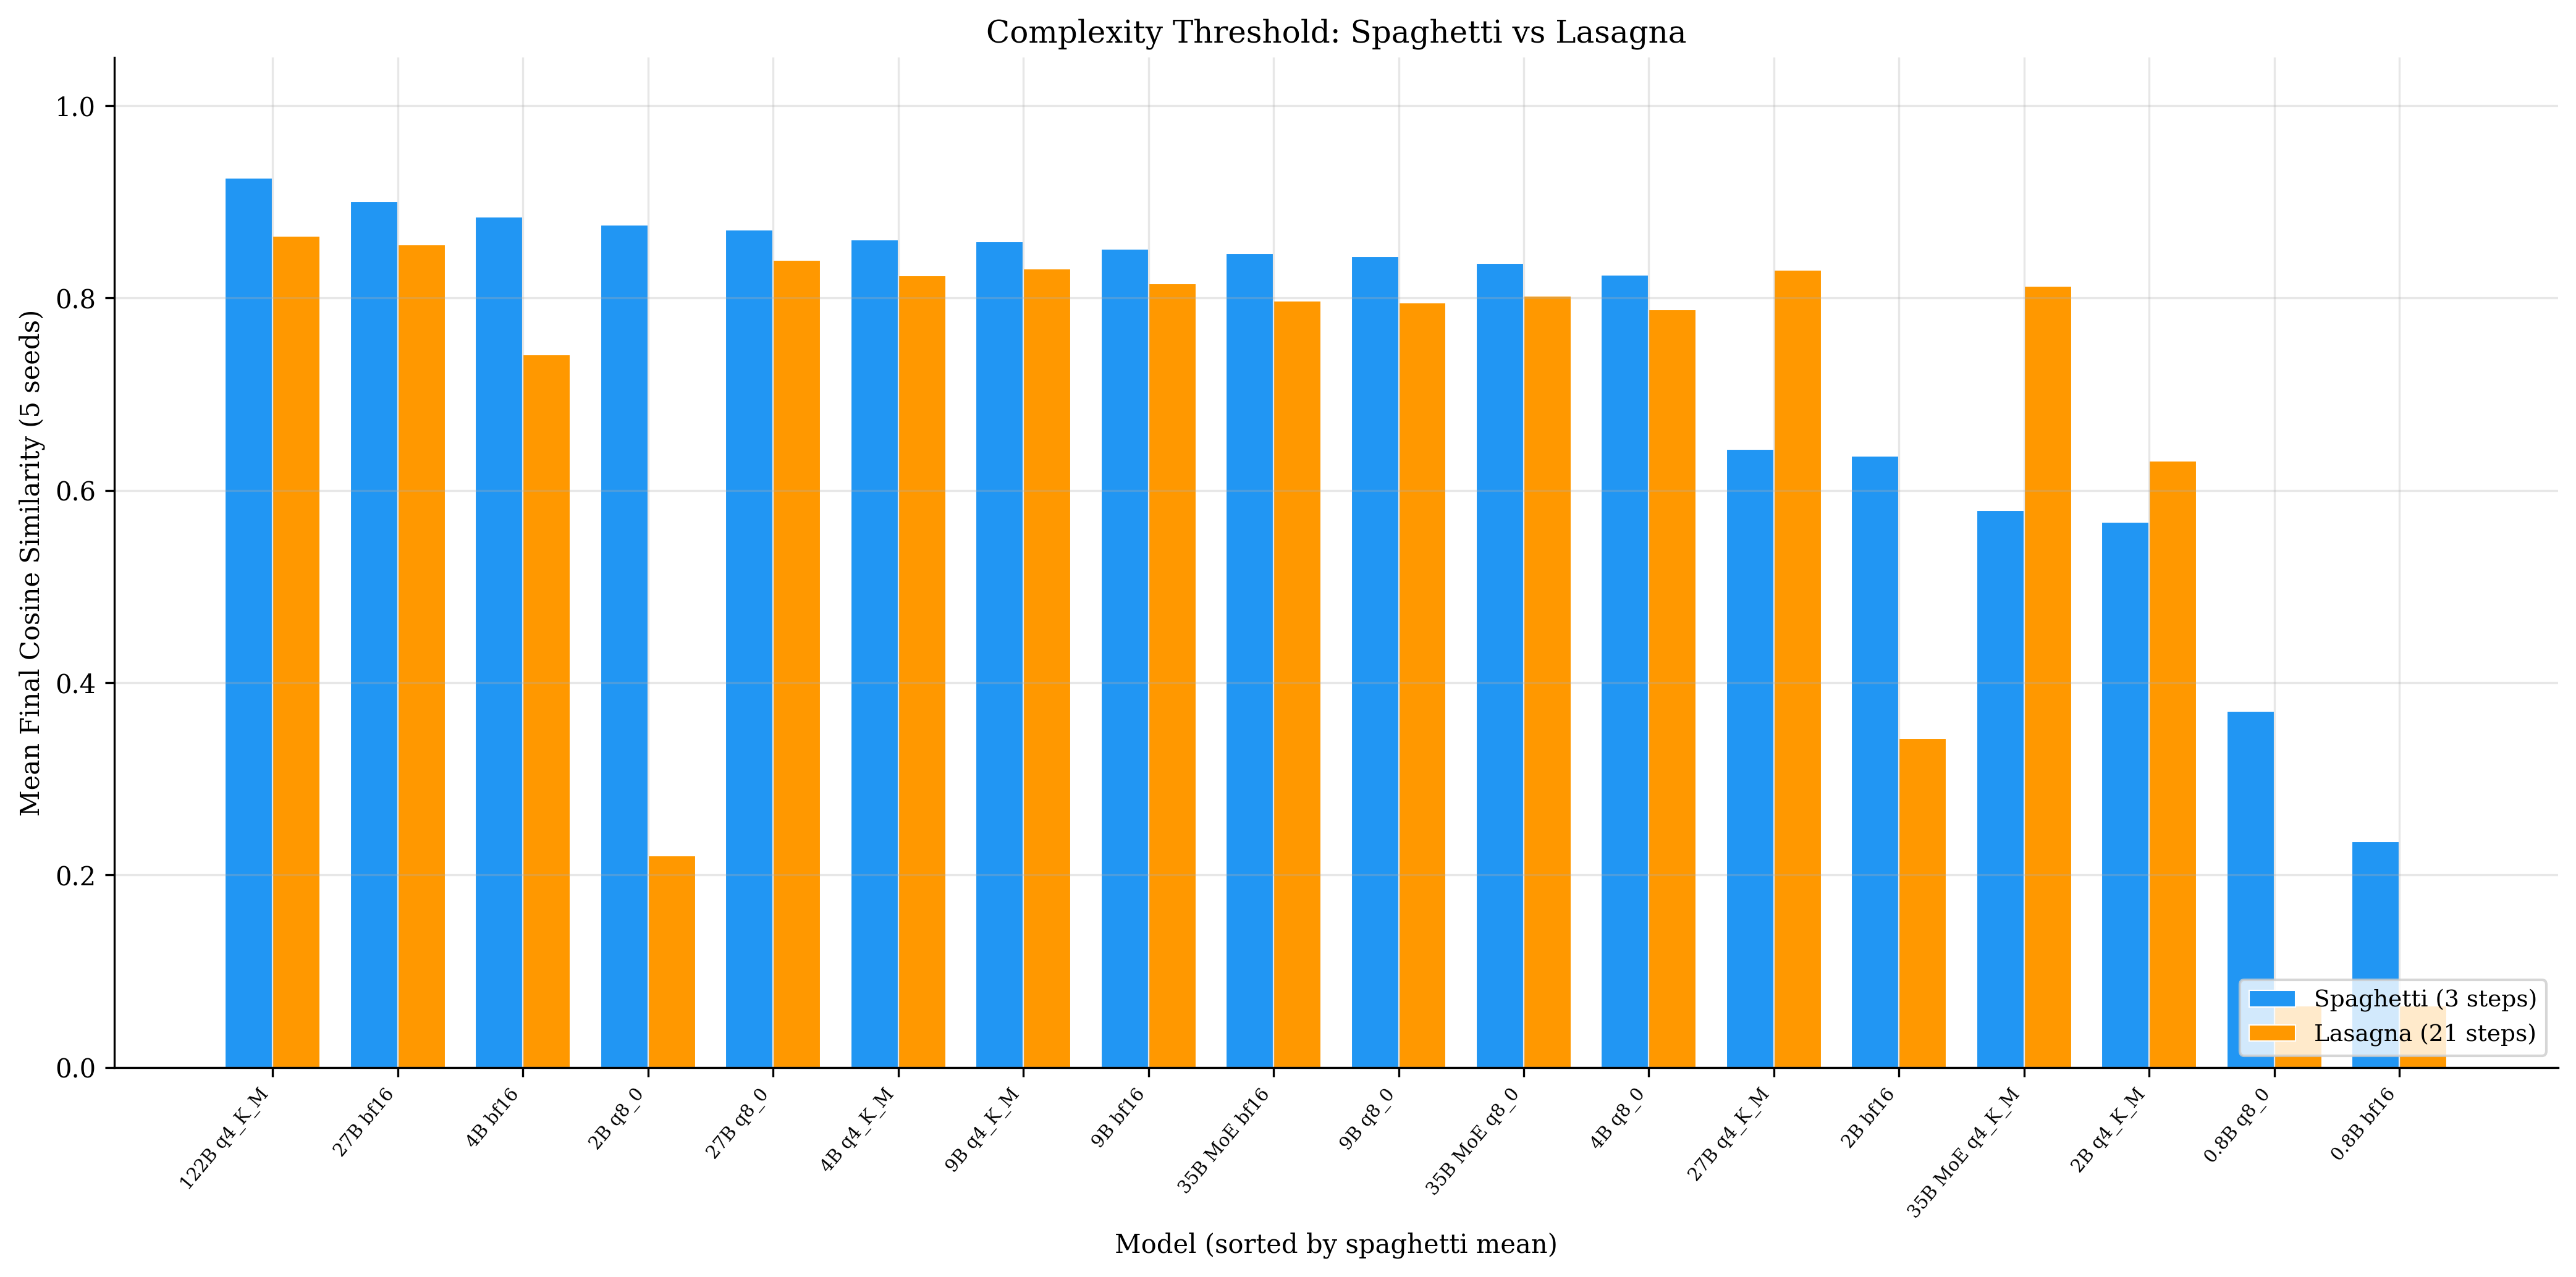
\includegraphics[width=\textwidth]{../results/qwen35_paper_figures/fig6_complexity_threshold.png}
\caption{Spaghetti (3 steps) vs.\ lasagna (21 steps) for all Qwen3.5
  models. Solid bars: spaghetti. Hatched bars: lasagna.}
\label{fig:complexity}
\end{figure}

Paper~1 found that system prompt effects only emerge with sufficiently
complex prompts. The Qwen3.5 data confirms the underlying asymmetry
between the two stimuli, and shows that it interacts with model size.
Among the models that are stable on spaghetti, the lasagna mean is
consistently the lower of the two but only modestly so
(122B: 0.925 vs.\ 0.864; 27B BF16: 0.900 vs.\ 0.855; 9B Q4\_K\_M:
0.859 vs.\ 0.830). Small models show far larger gaps---2B Q8\_0 drops
from 0.876 on spaghetti to 0.220 on lasagna, and both 0.8B variants fall
to 0.064---consistent with their struggling to carry a 21-step context
through iterated generation. The three configurations whose spaghetti
chains collapse into empty outputs (35B MoE Q4\_K\_M, 27B Q4\_K\_M,
2B Q4\_K\_M) invert the pattern and score \emph{higher} on lasagna,
which is a further indication that the short stimulus, not the long one,
is what triggers the empty-output failure mode.

\subsection{Cross-Generation Comparison}
\label{sec:crossgen}

Figure~\ref{fig:crossgen} compares Qwen3 and Qwen3.5 at matched
parameter counts using Q4\_K\_M quantization.

\begin{figure}[t]
\centering
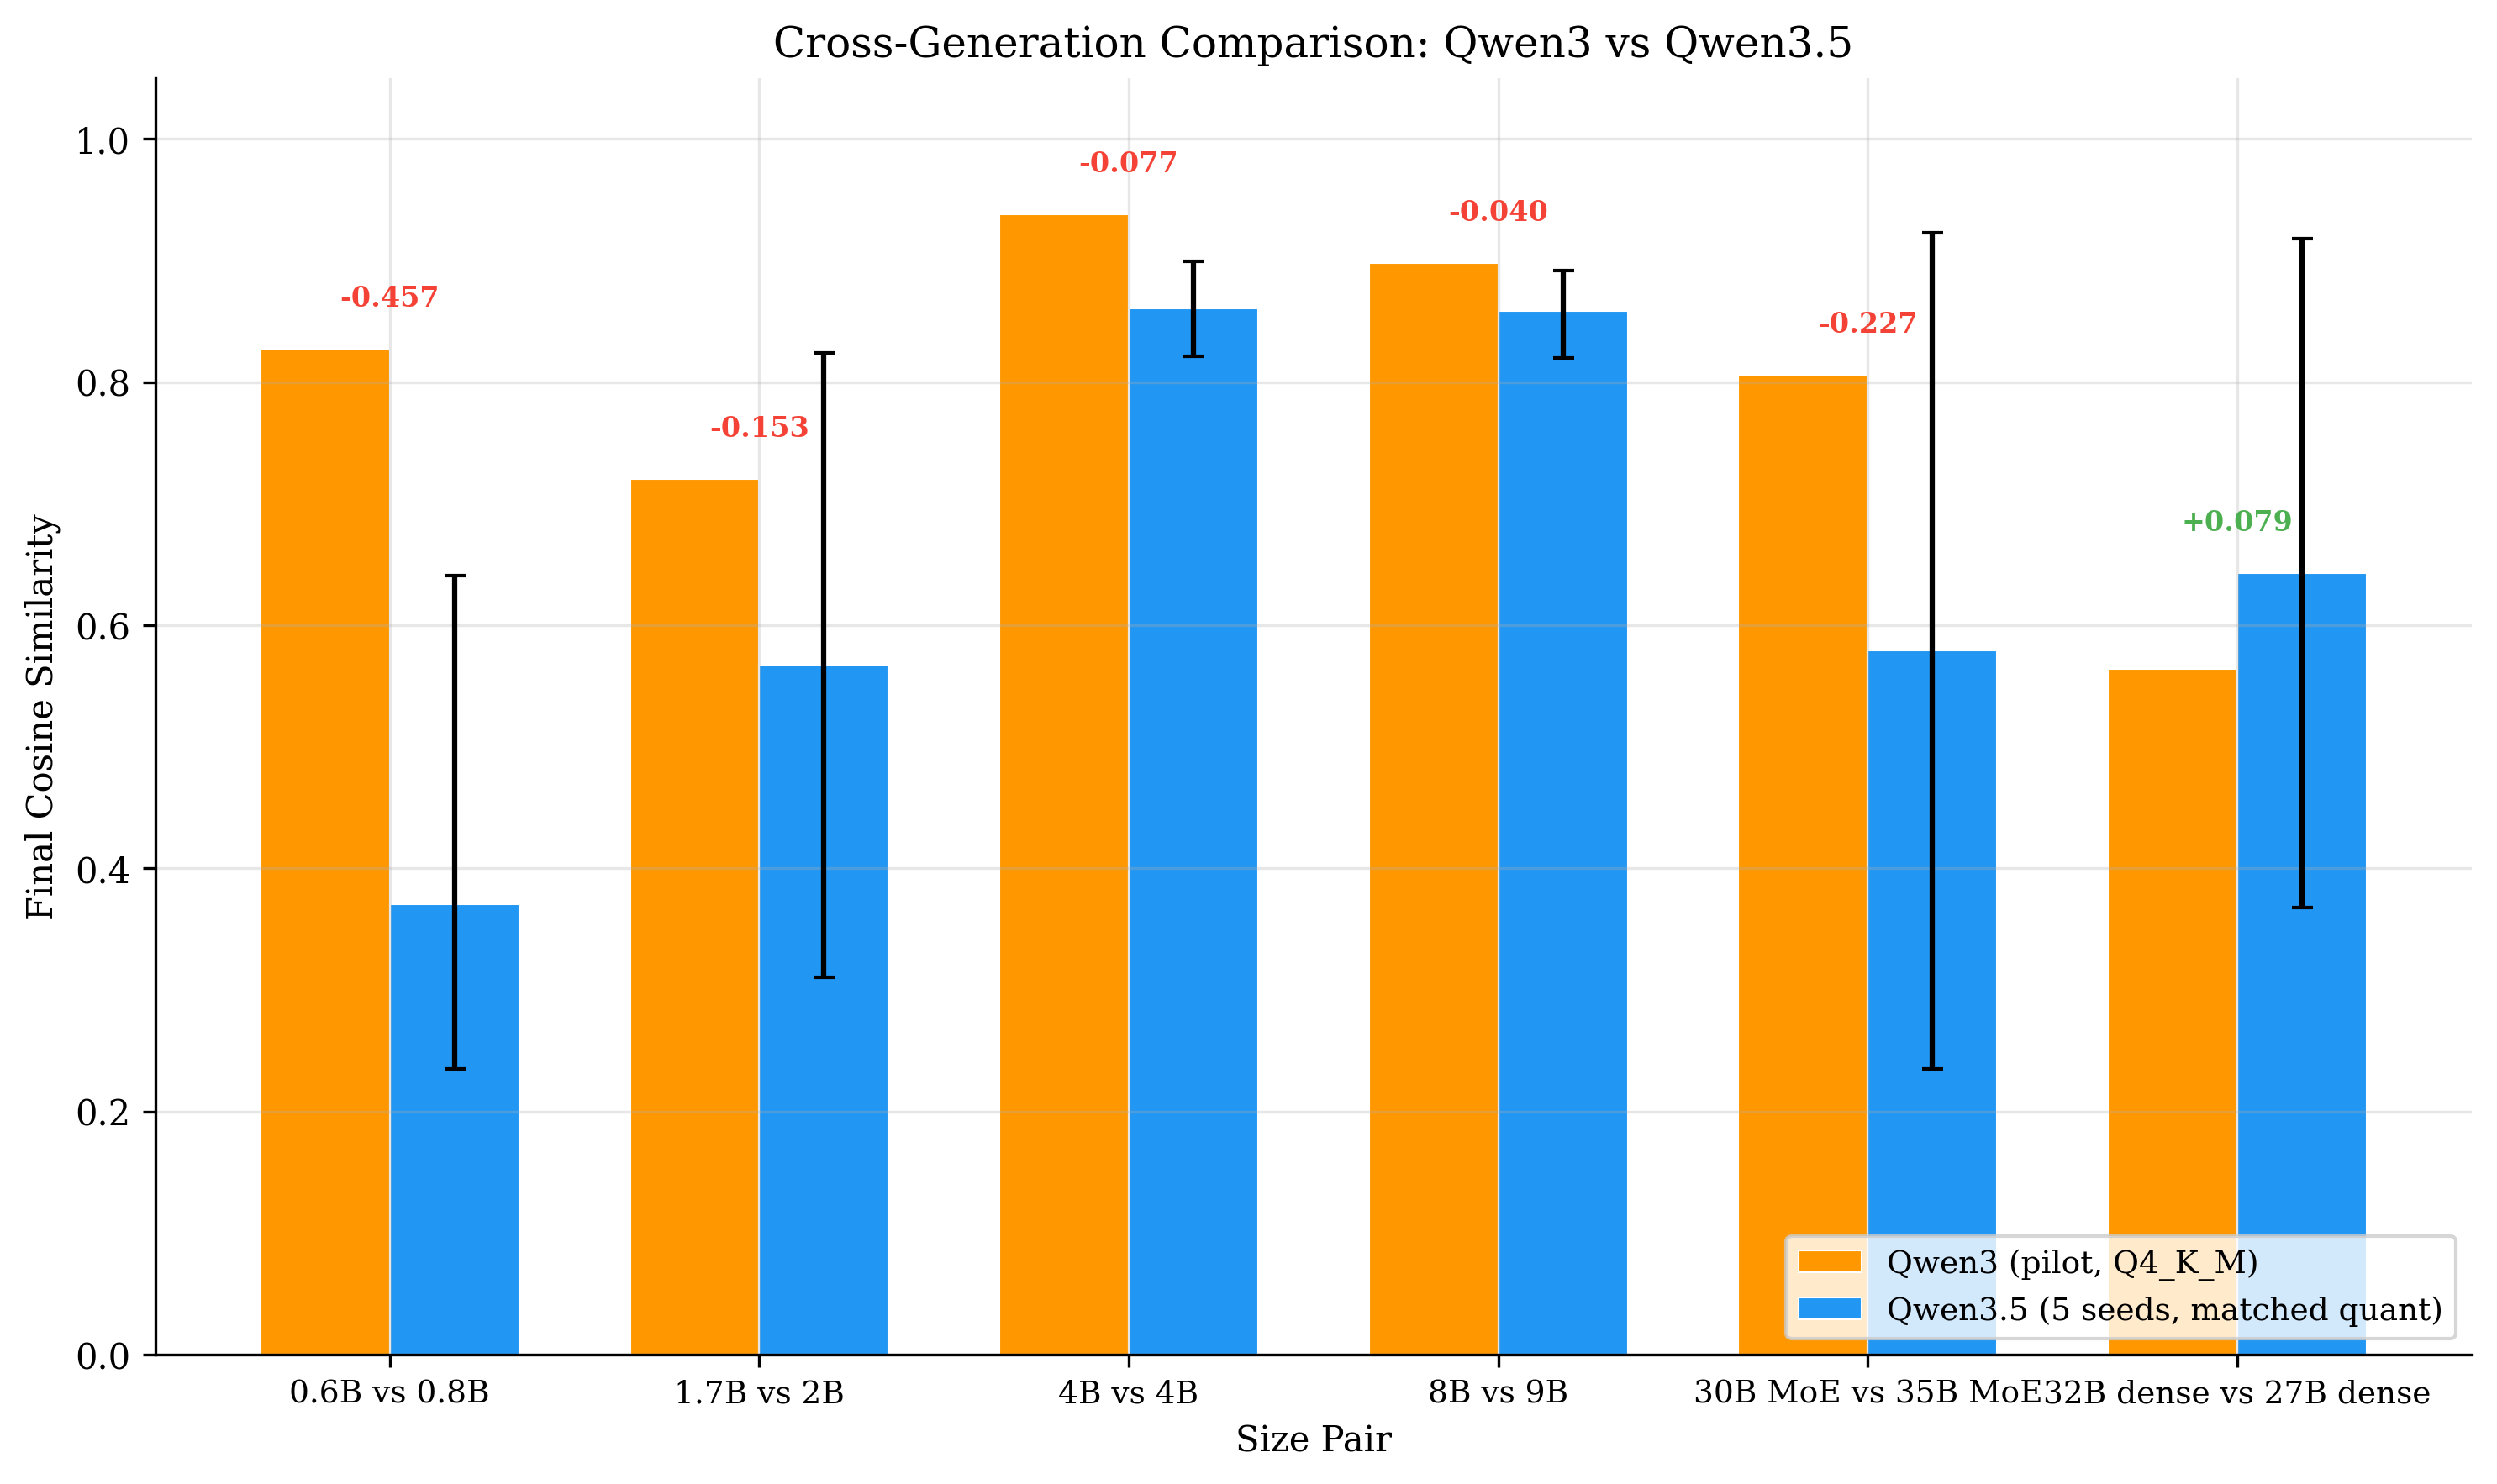
\includegraphics[width=0.85\textwidth]{../results/qwen35_paper_figures/fig10_cross_generation.png}
\caption{Cross-generation comparison: Qwen3 (pilot, single run) vs.\
  Qwen3.5 (up to 5 completed chains, matched quantization). The Qwen3
  bars carry \emph{no} error bars because each is a single unreplicated
  run from the Paper~1 pilot; only the Qwen3.5 bars have bootstrap CIs.}
\label{fig:crossgen}
\end{figure}

\paragraph{Dense model improvement at 27B.}
The 27B dense Qwen3.5 model is the only matched pair in which Qwen3.5
leads: 0.643 vs.\ Qwen3's 32B dense at 0.564 ($+$0.079). Its bootstrap
interval, [0.368, 0.918], comfortably contains the Qwen3 value, so this
is a directional observation rather than a demonstrated improvement.

\paragraph{MoE models regress.}
The 35B MoE (Qwen3.5, 0.579) trails the 30B MoE (Qwen3, 0.806) by
$-$0.227. Because the Qwen3.5 value is depressed by two chains that
collapse to the empty-output floor, this gap reflects a difference in
failure \emph{rate} rather than in gradual fidelity loss.

\paragraph{Small model regression.}
Below 4B parameters, Qwen3.5 regresses compared to Qwen3: the 0.8B model
(0.370) trails Qwen3's 0.6B (0.827) by $-$0.457, and the 2B (0.567)
trails Qwen3's 1.7B (0.720) by $-$0.153. The 4B and 9B pairs are close
to parity ($-$0.077 and $-$0.040). Taken together, five of six matched
pairs favour Qwen3. We caution strongly that the Qwen3 arm comes from a
single unreplicated pilot run with no confidence interval at all, while
the Qwen3.5 means are averaged over up to five chains; the comparison
should be read as motivating a properly seeded replication, not as
evidence of a generational regression.

% =============================================================================
% 5. DISCUSSION
% =============================================================================
\section{Discussion}
\label{sec:discussion}

\subsection{Comparison with Paper~1}

Paper~1 established a hierarchy of sensitivities: model choice $\gg$
infrastructure $>$ prompt engineering. The present within-family study
reveals a more nuanced picture:

\begin{enumerate}[leftmargin=*]
  \item \textbf{Size matters, but not monotonically.} The stability threshold
        at 4B confirms that model capacity is necessary but not sufficient.
        Above this threshold, the ordering is irregular: 4B BF16 (0.885)
        outperforms 9B Q8\_0 (0.844), and the 122B MoE (0.925) leads the
        best 35B MoE configuration (BF16, 0.846) by 0.079.
  \item \textbf{Quantization effects are architecture-dependent.}
        Paper~1 found that ``quantization is not monotonic.'' We confirm and
        strengthen this: the direction and magnitude of quantization effects
        depend on model size and on the failure mode involved. Among the
        small dense models the reversal is between BF16 and Q8\_0
        (2B: 0.876 for Q8\_0 vs.\ 0.636 for BF16); among the large models
        it is Q4\_K\_M that is anomalous, not because it degrades
        gradually but because it triggers whole-chain empty-output
        failures on the short stimulus.
  \item \textbf{Quantization method matters.} GGUF, AWQ, NVFP4 and
        GPTQ-Int4, despite all being 4-bit methods, produce different drift
        dynamics for the same 35B MoE weights. This extends Paper~1's
        Qwen3-VL finding to four quantization algorithms on the Qwen3.5
        family and suggests that the quantization algorithm itself---not
        just the precision---shapes multi-step behavior, though at
        $n\leq5$ chains per arm the individual pairwise intervals all
        include zero.
  \item \textbf{Temperature sensitivity inverts at small scales.} Paper~1
        found drift was ``not merely a function of sampling entropy.'' We
        find that for 2B models, the relationship between temperature and
        drift is actually \emph{inverted} at low temperatures, suggesting
        qualitatively different dynamics below the stability threshold.
\end{enumerate}

\subsection{Practical Implications}

For practitioners deploying Qwen3.5 in multi-agent pipelines:

\begin{itemize}[leftmargin=*]
  \item \textbf{Use $\geq$4B models.} Models below 4B are unreliable for
        iterative tasks, regardless of quantization.
  \item \textbf{Watch for empty-output collapse under Q4\_K\_M.} On the
        short stimulus, the 27B and 35B MoE Q4\_K\_M configurations
        returned empty completions for the majority of iterations in
        several chains. Monitor for empty responses explicitly rather than
        relying on an aggregate similarity score.
  \item \textbf{Test your quantization method.} GGUF, AWQ, NVFP4 and
        GPTQ-Int4 are not interchangeable for drift-sensitive
        applications; benchmark all candidate formats on representative
        tasks.
  \item \textbf{Avoid low temperatures with small models.} $T = 0.3$ can
        produce worse drift than $T = 1.0$ for 2B models.
\end{itemize}

\subsection{Limitations}

\begin{enumerate}[leftmargin=*]
  \item \textbf{Single model family.} Results may not generalize to other
        architectures (Llama, Gemma, etc.).
  \item \textbf{Paraphrase task only.} Other iterative tasks (summarization,
        translation) may show different patterns.
  \item \textbf{Embedding metric.} Validation against bge-m3 shows strong
        agreement ($r = 0.825$, $\rho = 0.815$), but 9.4\% of pairs
        were excluded due to bge-m3's shorter context window (8K vs.\ 32K
        tokens). All excluded pairs are highly-drifted outputs
        (see Appendix~\ref{app:embedding}).
  \item \textbf{Qwen3 comparison is unbalanced.} The Qwen3 data come from
        single pilot runs, while Qwen3.5 data have 5 seeds. The
        cross-generation comparison should be interpreted cautiously.
  \item \textbf{Seeds are samples, not replicates.} Paper~3 of this series
        establishes that fixing the sampling seed does not pin a chain
        under batched inference on these serving stacks: identical seeds
        can produce different trajectories because batch composition and
        kernel scheduling vary between requests. The five ``seeded'' runs
        behind each cell should therefore be read as five independent
        samples from the model's output distribution, not as reproducible
        replicates. All bootstrap intervals here are intervals over those
        samples.
  \item \textbf{The lasagna stimulus is compressed.} The 21-step recipe
        actually sent to the models collapses steps 12--17 into the single
        line ``Step 12--17: Layer sauce, noodles, ricotta, mozzarella
        (3 layers).'' It is therefore a 16-line stimulus that nominally
        spans 21 steps (Appendix~\ref{app:prompts}). Results for the
        ``21-step'' condition should be read accordingly.
  \item \textbf{Incomplete conditions.} Thirty-eight of the 2{,}007 chains
        did not reach iteration~30 and are excluded from every statistic
        (Section~\ref{sec:method}). Three of the affected serving
        endpoints have since been retired, so these conditions cannot be
        regenerated with the same software stack.
  \item \textbf{Empty outputs and thinking overhead.} Several models
        (particularly 0.8B and 27B Q4\_K\_M) produce empty output strings
        in a substantial fraction of iterations. We attribute this to
        Qwen3.5's think-before-responding architecture consuming the
        generation budget on internal reasoning tokens, but we cannot
        fully rule out serving-layer issues (e.g., Ollama silently
        truncating). The empty outputs are recorded as data and chains
        continue with the previous non-empty message, but this recovery
        mechanism may mask the true depth of drift.
\end{enumerate}

% =============================================================================
% 6. CONCLUSION
% =============================================================================
\section{Conclusion}
\label{sec:conclusion}

We have presented the first controlled within-family analysis of semantic
drift in iterated LLM paraphrase chains, studying the Qwen3.5 model family
across 7 parameter sizes, 18 size/quant combinations, three serving
backends (Ollama/GGUF, vLLM/AWQ and GPTQ-Int4, sglang/NVFP4), 5
temperatures, and 20 system prompts, in 1{,}969 completed 30-iteration
chains totalling 59{,}070 inferences. Our key findings are:

\begin{enumerate}[leftmargin=*]
  \item A stability threshold at approximately 4B parameters, below which
        drift behavior becomes unpredictable.
  \item Non-monotonic, size-dependent quantization effects, in which the
        ordering of BF16, Q8\_0 and Q4\_K\_M reverses between model sizes.
  \item Measurable differences between GGUF, AWQ, NVFP4 and GPTQ-Int4
        quantization methods for the same underlying architecture, with the
        caveat that at $n\leq5$ chains per arm the pairwise intervals
        overlap.
  \item Inverted temperature sensitivity in small models, where low
        temperatures produce \emph{worse} drift than high temperatures.
  \item A cross-generation comparison in which five of six matched pairs
        favour Qwen3 over Qwen3.5, which we report as a call for a properly
        seeded replication given that the Qwen3 arm is a single pilot run.
\end{enumerate}

These findings refine Paper~1's sensitivity hierarchy: within a single
model family, \emph{size} dominates \emph{quantization}, which dominates
\emph{temperature} and \emph{prompt engineering}. However, the interactions
between these factors are complex and non-monotonic, underscoring the need
for empirical benchmarking of specific model configurations in
drift-sensitive applications.

% =============================================================================
% REFERENCES
% =============================================================================
\bibliographystyle{plainnat}
\bibliography{references}

% =============================================================================
% APPENDICES
% =============================================================================
\clearpage
\appendix

\section{Prompt Texts}
\label{app:prompts}

\subsection{Spaghetti (3 steps)}
\begin{quote}
Step 1: Boil water. Step 2: Add pasta for 8 minutes. Step 3: Drain and
serve with sauce.
\end{quote}

\subsection{Lasagna (nominally 21 steps)}

The following is the \emph{verbatim} stimulus string sent to the models
(\texttt{PROMPTS["lasagna"]} in \texttt{scripts/\allowbreak run\_qwen35\_\allowbreak size\_quant.py}).
Note that although the recipe is numbered through step~21, steps 12--17 are
compressed into a single line in the stimulus itself, so the text actually
transmitted contains 16 lines rather than 21. We reproduce it exactly rather
than expanding it, because the compression is part of the condition being
measured.

\begin{quote}
\small
Follow these exact steps to prepare a classic homemade beef lasagna that
serves 8-10 people:
Step 1: Preheat your oven to 375\textdegree F (190\textdegree C) and lightly
grease a 9$\times$13 inch baking dish.
Step 2: Bring a large pot of lightly salted water to a boil.
Step 3: Heat 2 tablespoons of olive oil in a large skillet over medium heat.
Step 4: Add 1 large finely diced onion and cook for 5 minutes until
translucent.
Step 5: Add 5 minced garlic cloves and cook for 1 minute until fragrant.
Step 6: Add 1.25 lbs ground beef and 0.75 lb Italian sausage. Cook until
browned.
Step 7: Drain excess grease from the skillet.
Step 8: Stir in two 28-oz cans of crushed tomatoes, 3 tbsp tomato paste,
2 tsp dried basil, 1.5 tsp dried oregano, 0.5 tsp fennel seed, 1 tsp sugar,
1 tsp salt, and 0.5 tsp black pepper.
Step 9: Bring to a simmer and cook the meat sauce for 30 minutes.
Step 10: Combine 15 oz ricotta, 1 egg, 1/2 cup Parmesan, 1/4 cup parsley,
1/2 tsp salt, 1/4 tsp pepper.
Step 11: Cook 12 lasagna noodles until al dente. Drain and rinse.
Step 12-17: Layer sauce, noodles, ricotta, mozzarella (3 layers).
Step 18: Cover with foil and bake 25 minutes.
Step 19: Remove foil and bake 25-30 more minutes until golden.
Step 20: Rest 15-20 minutes before slicing.
Step 21: Garnish with fresh basil and serve hot.
\end{quote}

The spaghetti stimulus given above is likewise reproduced verbatim from
\texttt{PROMPTS["spaghetti"]} in the same file.

\section{Model Inventory}
\label{app:models}

All GGUF models were served with Ollama on a single on-premises GPU
server. The vLLM models were
\texttt{cyankiwi/\allowbreak Qwen3.5-35B-A3B-AWQ-4bit} (AWQ 4-bit),
\texttt{Qwen/\allowbreak Qwen3.5-35B-A3B-GPTQ-Int4} (GPTQ-Int4) and
\texttt{cyankiwi/\allowbreak Qwen3.5-9B-AWQ-4bit} (9B AWQ). The sglang models were
\texttt{txn545/\allowbreak Qwen3.5-35B-A3B-NVFP4} and, as the out-of-family control,
\texttt{nvidia/\allowbreak NVIDIA-\allowbreak Nemotron-\allowbreak 3-Nano-\allowbreak 30B-A3B-\allowbreak NVFP4}. Similarity was
computed with Qwen3-Embedding-0.6B served by vLLM. Hardware and software
versions are given in Appendix~\ref{app:compute}.

Note: Qwen3.5 0.8B Q4\_K\_M does not exist as a released quantization.
Qwen3.5 122B is only available in Q4\_K\_M due to GPU memory constraints.
No official GPTQ-Int4 build of Qwen3.5 9B exists, and the available 9B
NVFP4 builds come from publishers other than the one used for the 35B
NVFP4 model, so a 9B NVFP4 arm was excluded to avoid a calibration
confound.

\section{Additional Figures}
\label{app:figures}

\begin{figure}[h]
\centering
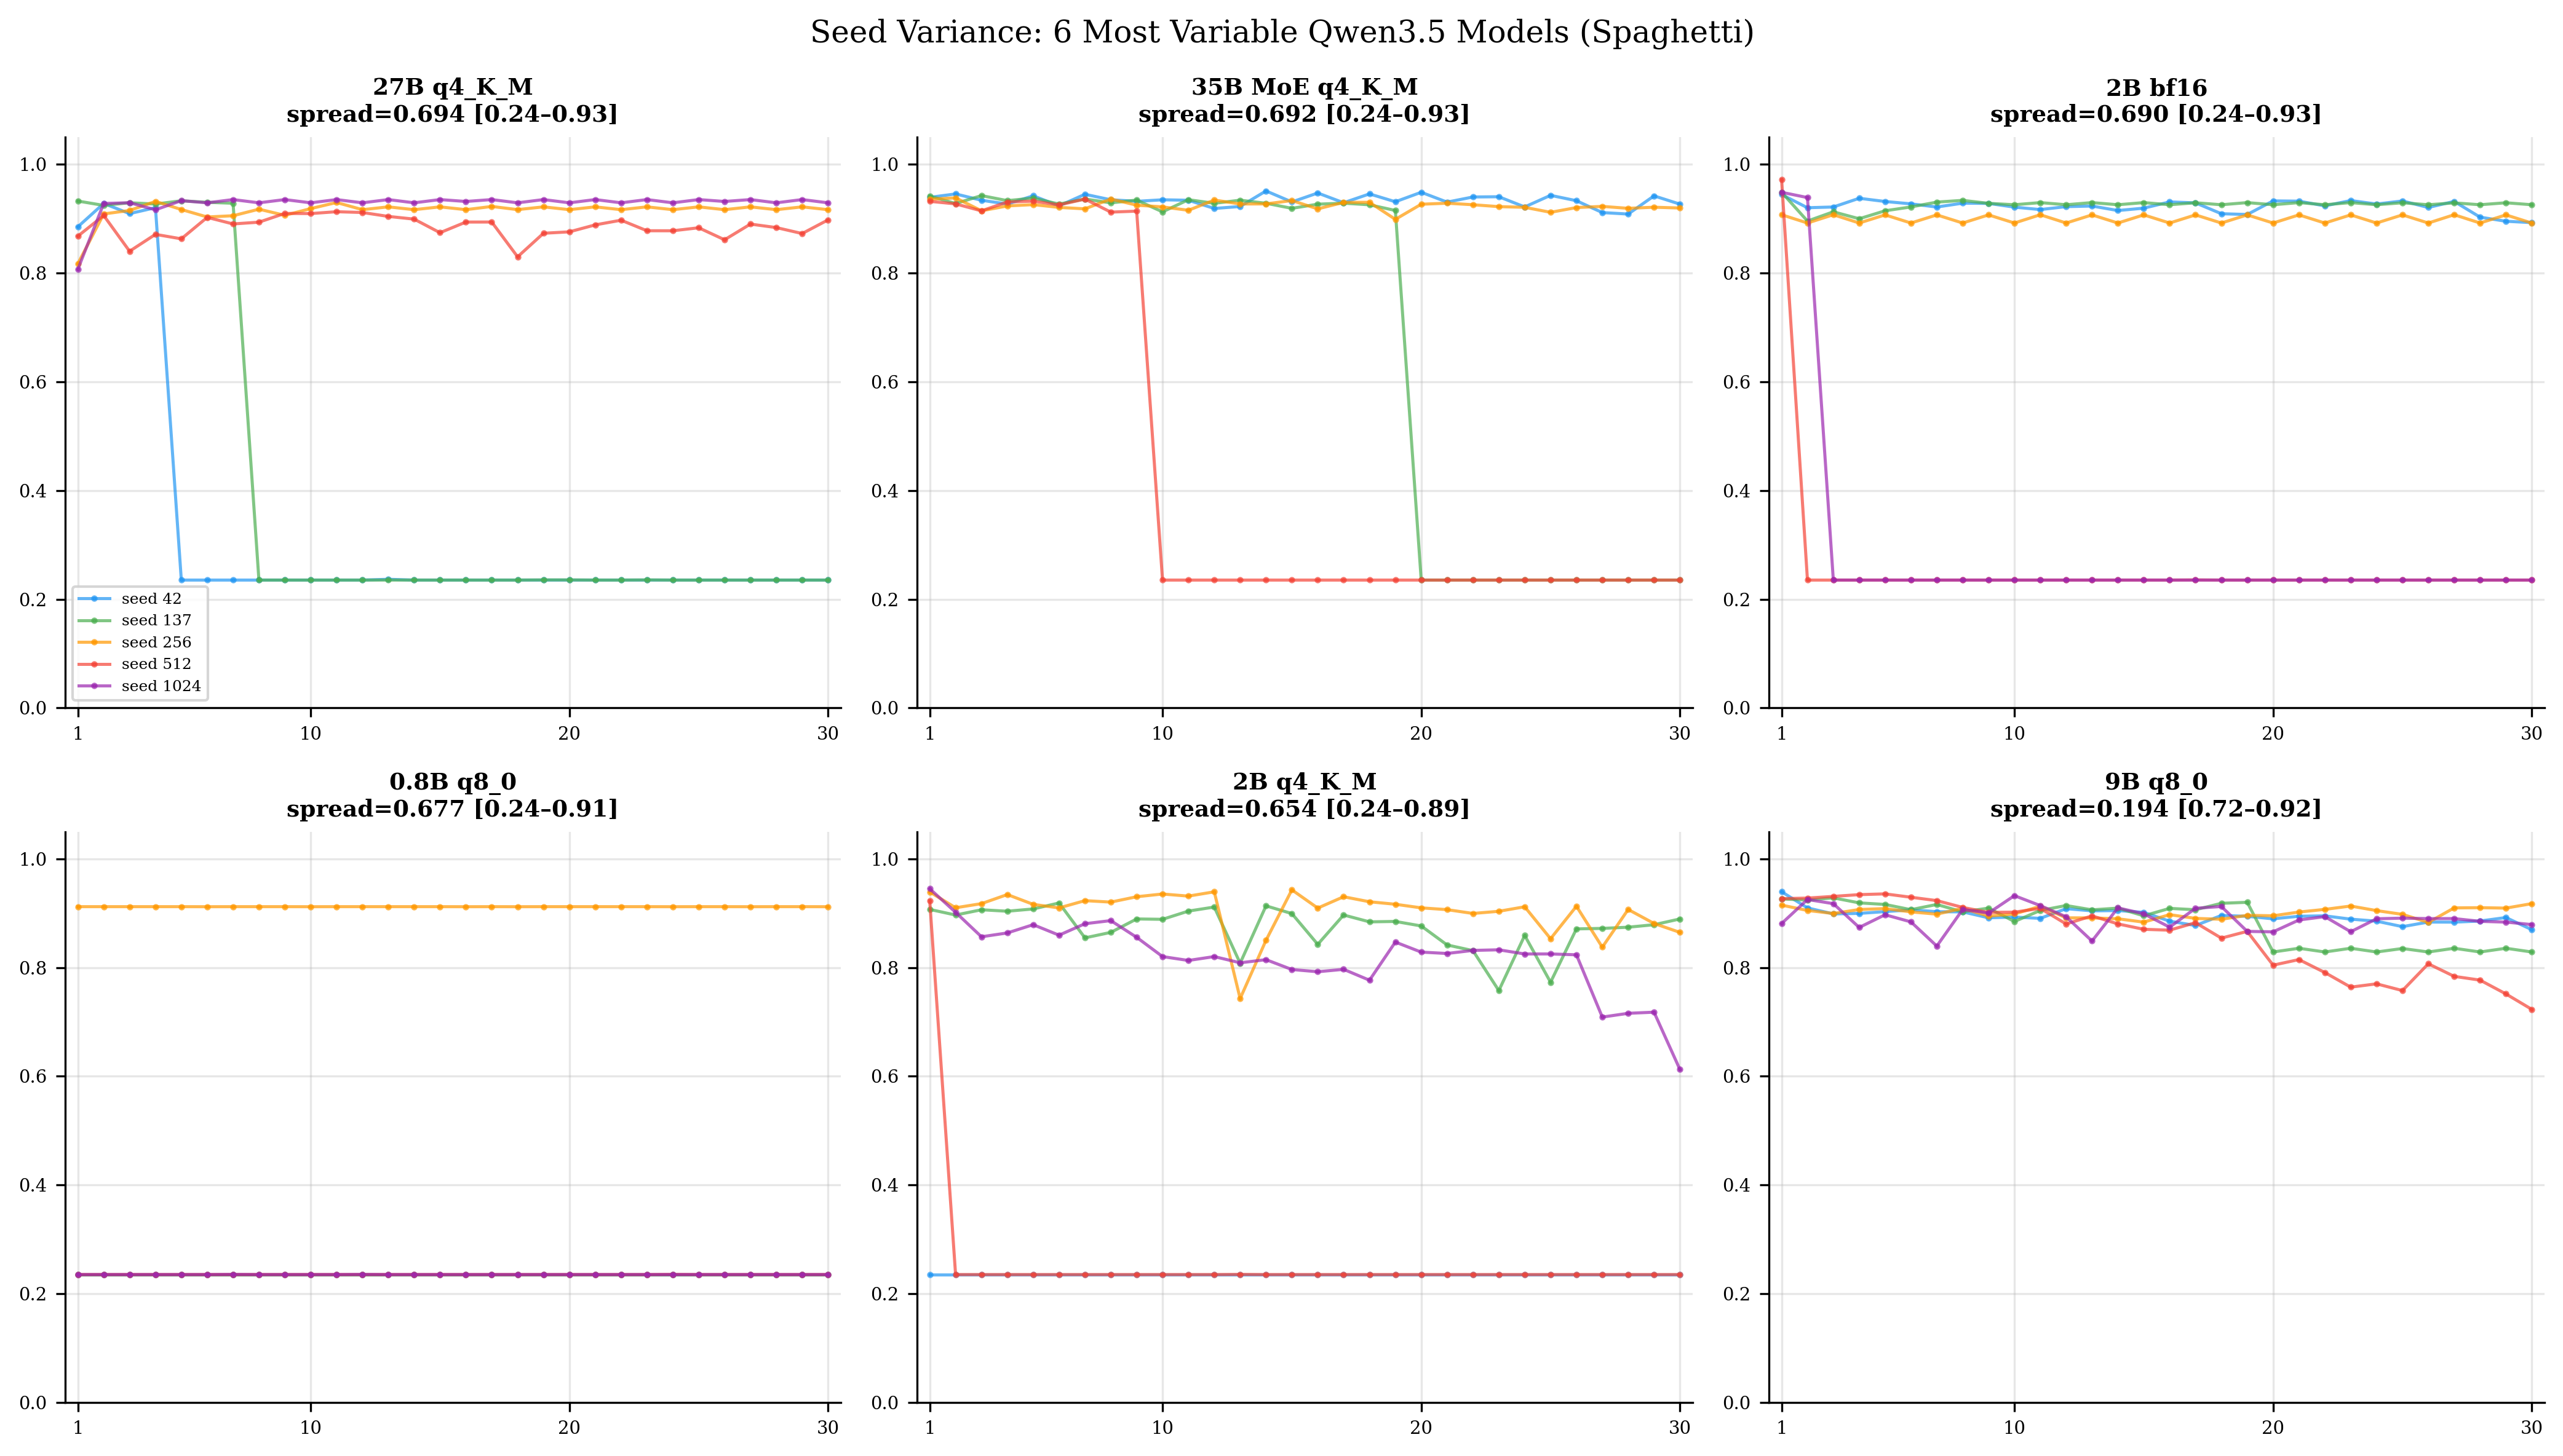
\includegraphics[width=\textwidth]{../results/qwen35_paper_figures/figA2_seed_variance.png}
\caption{Seed variance for the 6 most variable Qwen3.5 models on the
  spaghetti recipe. Individual seed trajectories shown.}
\label{fig:seed_var}
\end{figure}

\begin{figure}[h]
\centering
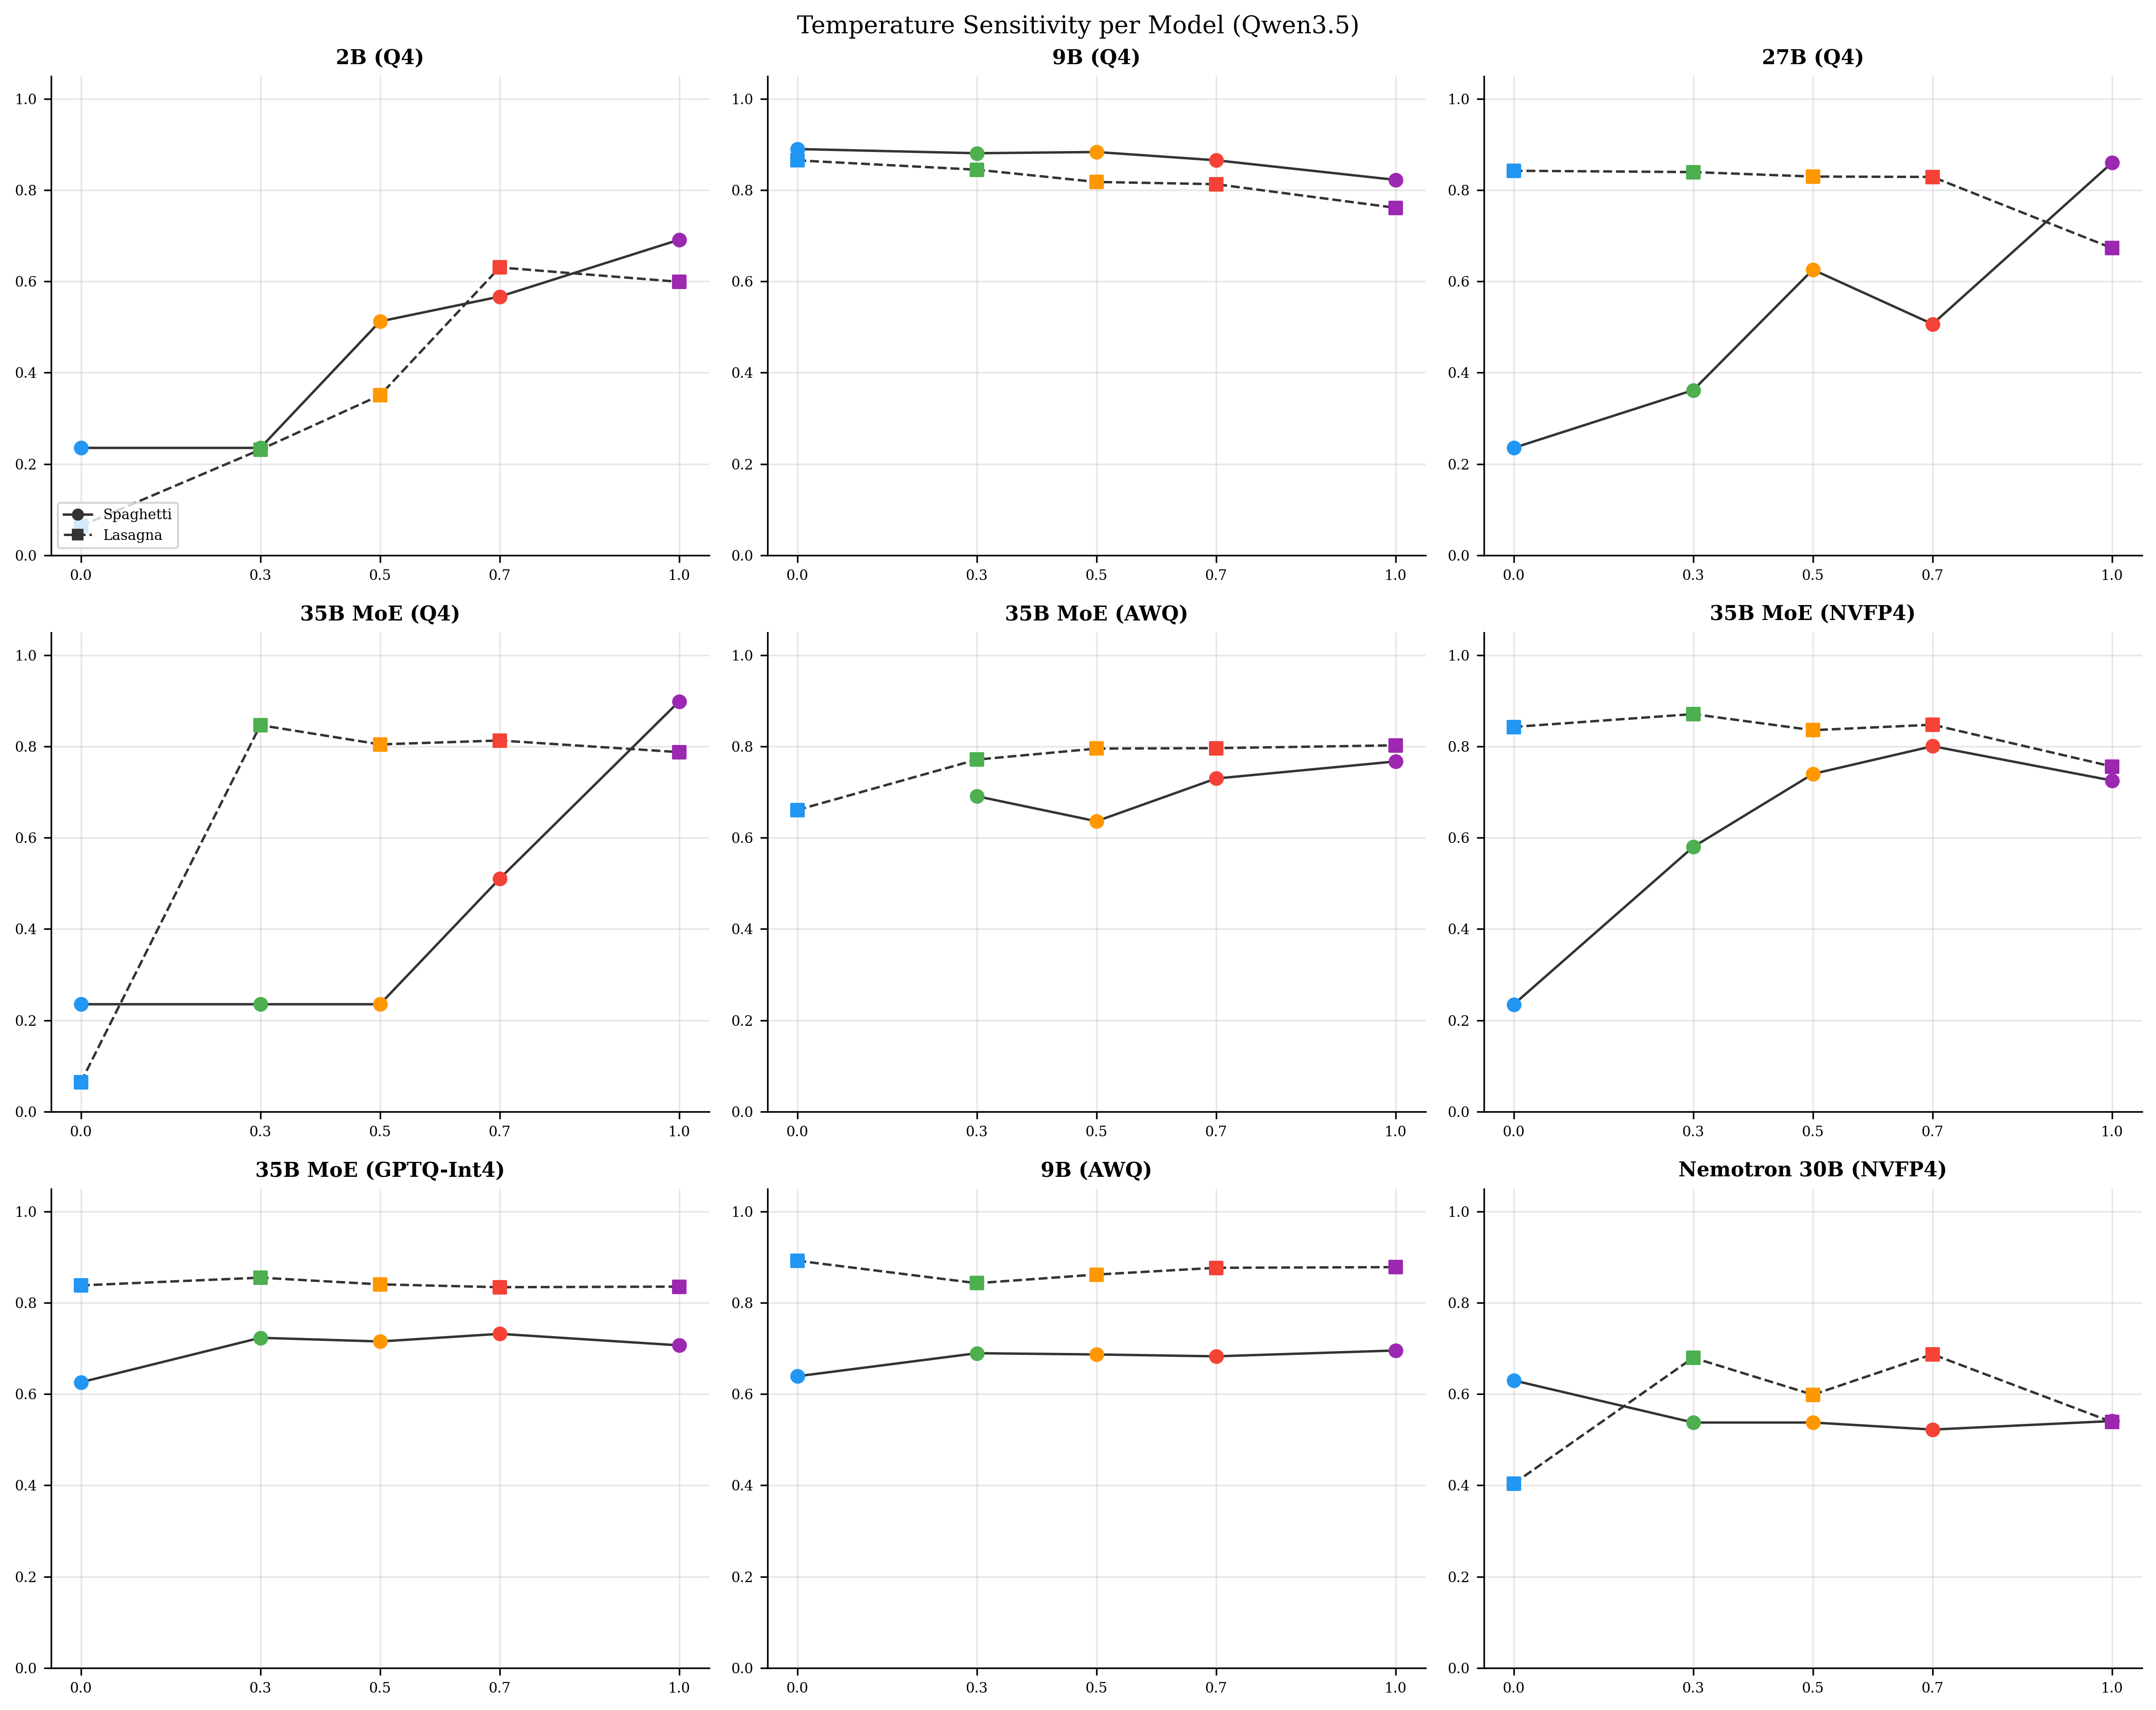
\includegraphics[width=0.85\textwidth]{../results/qwen35_paper_figures/figA3_temperature_multiples.png}
\caption{Temperature sensitivity per model: mean final similarity at each
  temperature for spaghetti (solid) and lasagna (dashed).}
\label{fig:temp_multi}
\end{figure}

\section{Embedding Model Validation}
\label{app:embedding}

Following Paper~1, we validate our primary embedding model
(Qwen3-Embedding-0.6B, 32{,}768-token context) against bge-m3
(8{,}192-token context) by re-embedding all text pairs from the Qwen3.5
experiments and computing Pearson and Spearman correlations between the two
models' cosine similarity scores.

Of 22{,}167 total pairs, 20{,}072 (90.6\%) produced valid similarities from
both models, yielding Pearson $r = 0.825$ and Spearman $\rho = 0.815$
($p < 10^{-10}$ for both). This strong agreement validates that our drift
measurements are not artifacts of the specific embedding model chosen.

The remaining 2{,}095 pairs (9.4\%) failed because bge-m3's vLLM endpoint
rejects inputs exceeding its 8{,}192-token context window rather than
truncating them. All failed pairs are outputs exceeding 6{,}000 words,
produced by chains that experienced runaway text expansion---a
characteristic drift failure mode where certain system prompts
(e.g., ``Visual Tutorial Style,'' ``Friendly Conversational'') cause
outputs to grow by several thousand words over 30 iterations. These
excluded pairs have a mean Qwen similarity of 0.515 (median 0.572)
compared to the dataset mean of 0.829, confirming they are systematically
the most-drifted outputs. Because both embedding models would score these
highly-diverged texts as low similarity, their exclusion is unlikely to
meaningfully affect the correlation.

\begin{figure}[h]
\centering
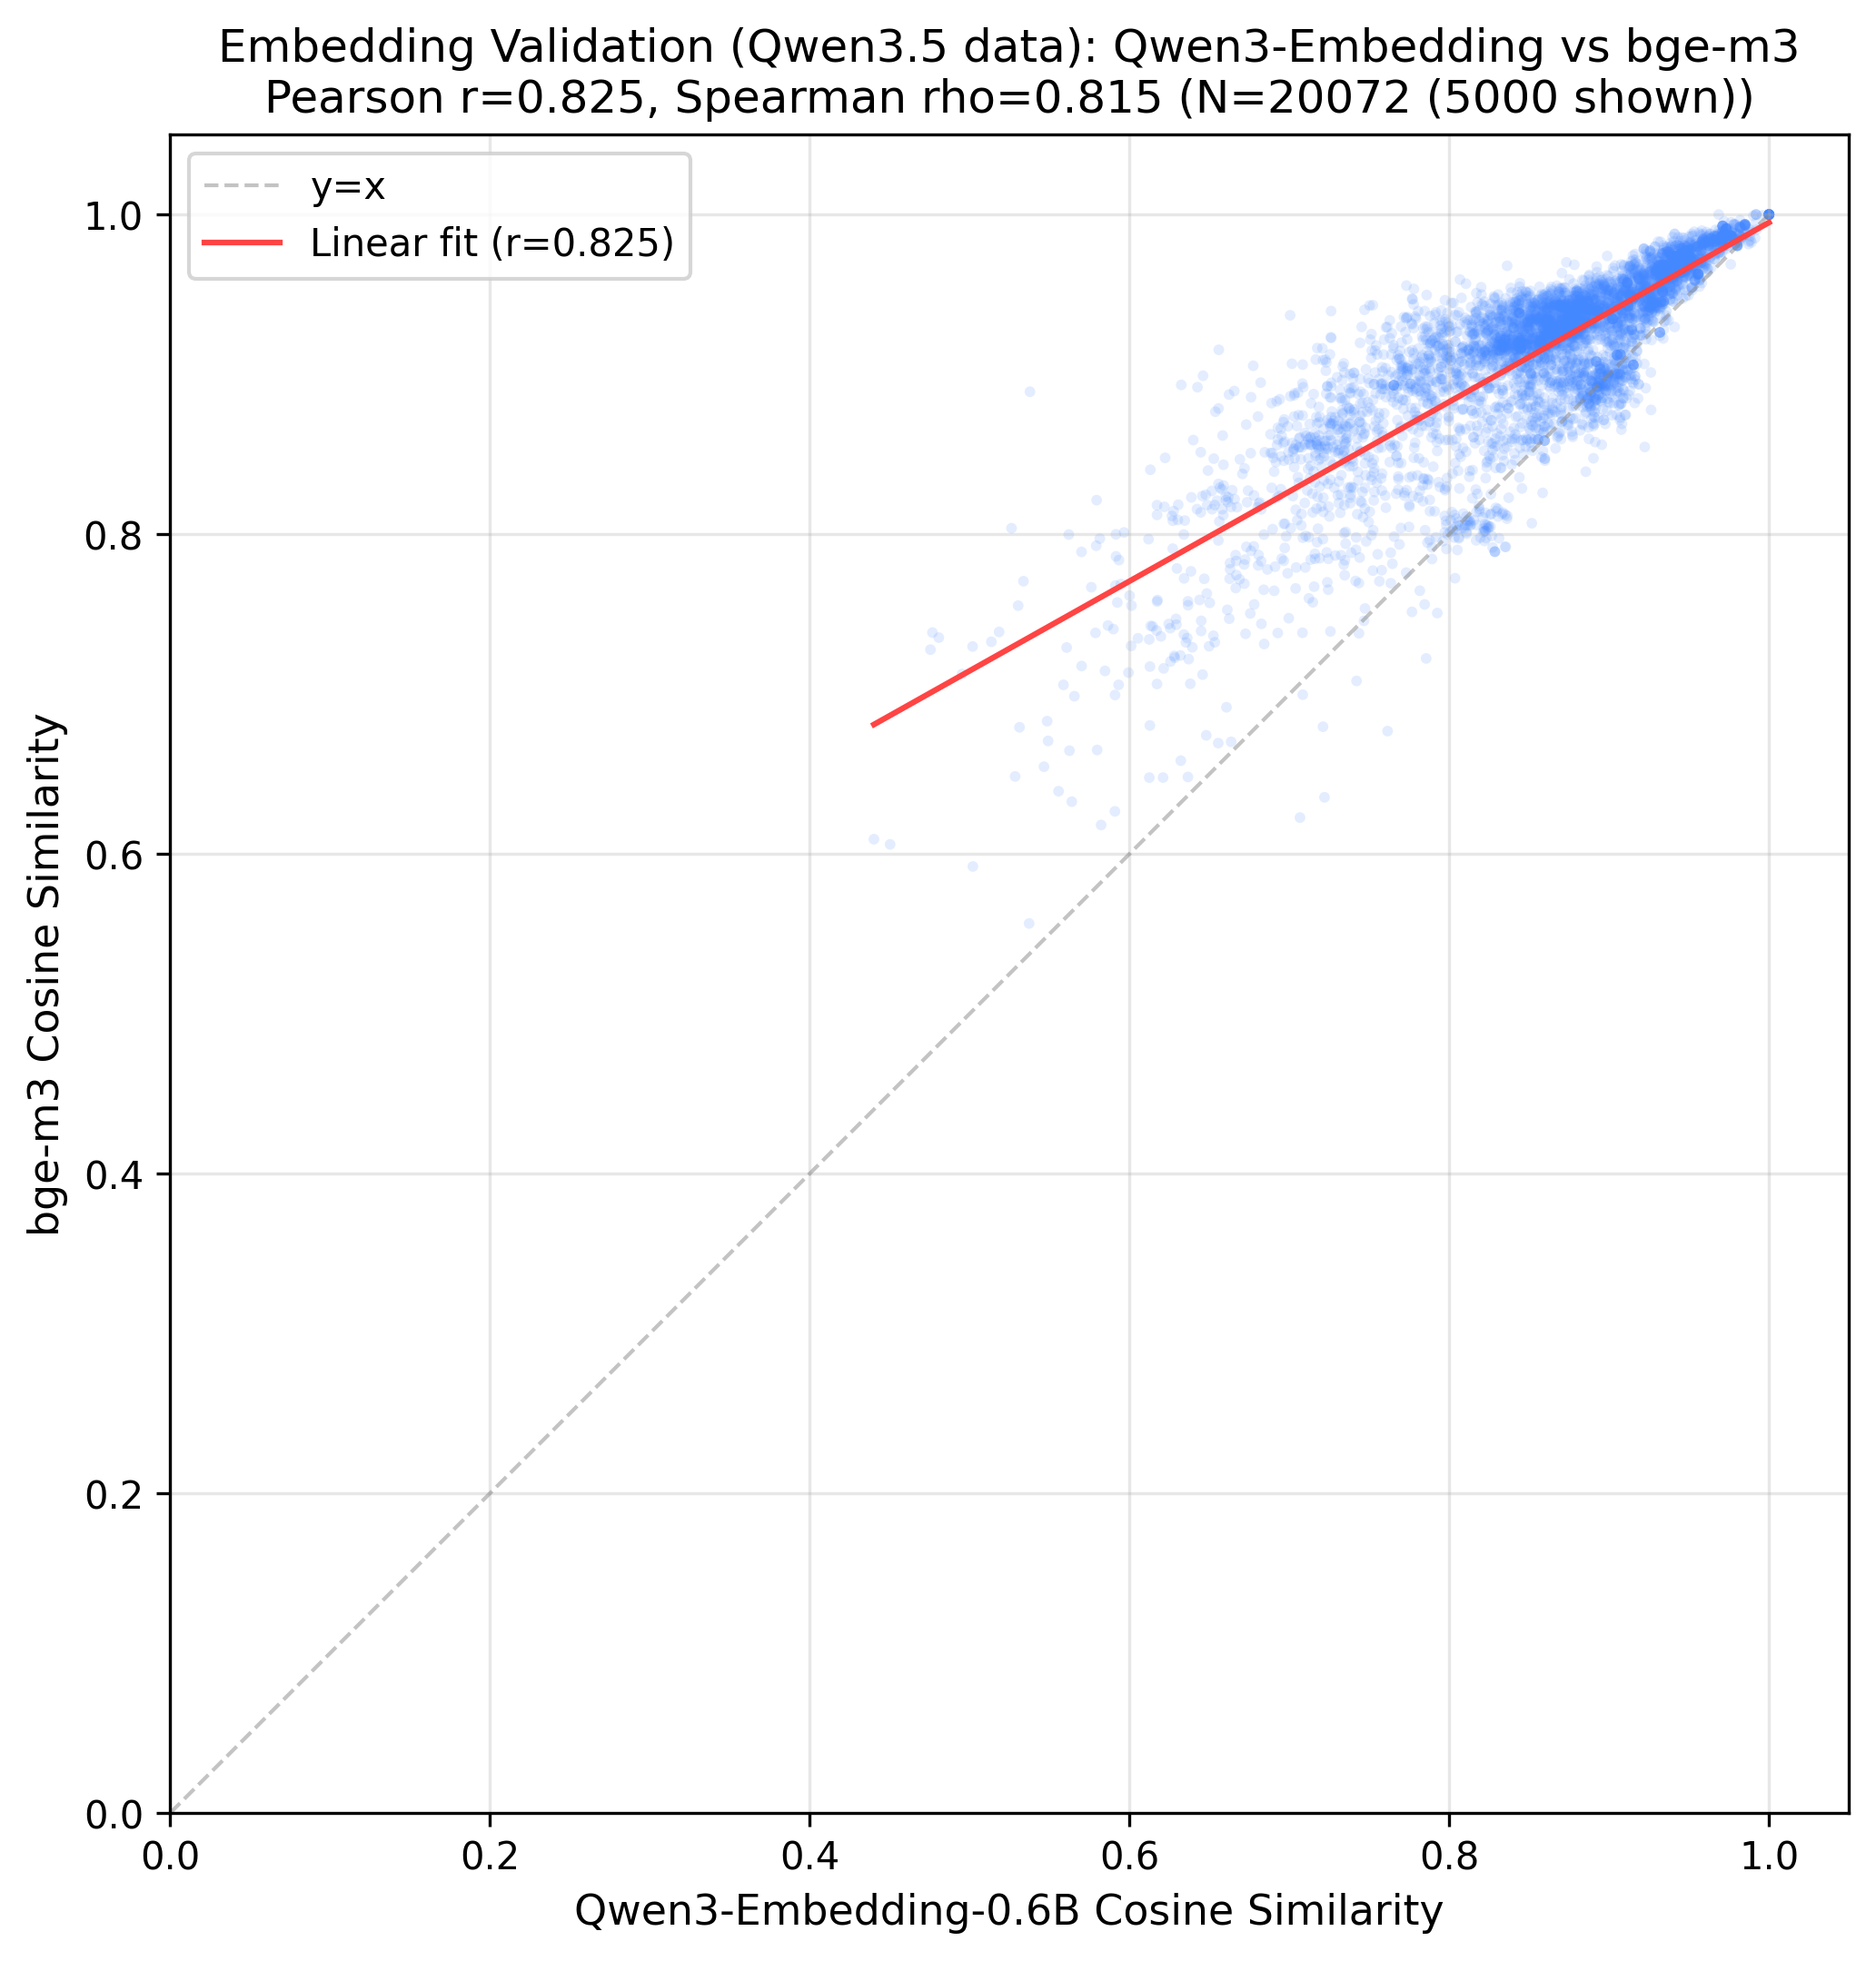
\includegraphics[width=0.75\textwidth]{../results/embedding_validation_qwen35/embedding_scatter.png}
\caption{Embedding model validation scatter: Qwen3-Embedding-0.6B vs.\
  bge-m3 cosine similarities for 20{,}072 Qwen3.5 experiment text pairs
  (2{,}095 pairs with outputs exceeding bge-m3's 8{,}192-token context
  limit excluded). Pearson $r = 0.825$, Spearman $\rho = 0.815$.}
\label{fig:embed_val}
\end{figure}

\section{Reproducibility and Compute}
\label{app:compute}

\paragraph{Hardware.}
All Ollama and vLLM runs were executed on a single on-premises server with
one NVIDIA RTX~PRO~6000 Blackwell GPU (96\,GB). The sglang NVFP4 runs
(35B NVFP4 and the Nemotron control) were executed on a second on-premises
server with one NVIDIA RTX~5090 GPU (32\,GB). Embeddings were computed with
Qwen3-Embedding-0.6B served by vLLM on the same infrastructure.

\paragraph{Software.}
Ollama v0.16.3; vLLM v0.15.1, plus a CUDA~13.0 nightly build of vLLM for the
GPTQ-Int4 and 9B~AWQ runs; sglang for the NVFP4 runs. Analysis used Python
with NumPy, SciPy and Matplotlib, driven by
\texttt{scripts/\allowbreak analyze\_qwen35\_paper.py}; dependencies are pinned with
\texttt{uv}.

\paragraph{Scale and compute budget.}
The study comprises 1{,}969 completed 30-iteration chains, that is 59{,}070
LLM inferences, drawn from 2{,}007 launched chains. Summing the recorded
per-iteration wall-clock times across all Paper~2 data files gives
approximately 630 hours of cumulative inference time; because several
experiments ran with up to four concurrent workers, the elapsed wall-clock
duration of the campaign was substantially shorter than that figure.
Embedding validation added a further 22{,}167 embedding pairs
(Appendix~\ref{app:embedding}).

\paragraph{Availability.}
The experiment scripts, raw per-iteration drift records and the analysis
code that produces every figure and table in this paper are available from
the author on request; a public repository will be linked here once one is
released.

\end{document}
